\documentclass{beamer}
% \documentclass[10pt]{beamer}
% \documentclass[aspectratio=169]{beamer}

\usepackage[utf8]{inputenc}
%\usepackage{lmodern}
\usepackage{comment}
\usetheme{Madrid}
\usepackage{csquotes}
\usepackage[maxbibnames=99,backend=biber,style=ieee,doi=false,isbn=false,eprint=false]
{biblatex}
% \usepackage[maxbibnames=99,backend=biber,style=ieee,doi=false,isbn=false,eprint=false,url=false]{biblatex}
\addbibresource{references.bib}
\definecolor{cvut_navy}{HTML}{0065BD}
\definecolor{cvut_blue}{HTML}{6AADE4}
\definecolor{cvut_gray}{HTML}{156570}
\definecolor{faeng_blue}{HTML}{09246F}
%\usepackage{tikz}
%\usepackage{pgfplots}
\usepackage{textcomp}

\usepackage[makeroom]{cancel}
\usepackage{threeparttable}
\usepackage[utf8]{inputenc}
%\usepackage[usenames,dvipsnames]{xcolor}
\setbeamercolor{section in toc}{fg=black,bg=yellow}
\setbeamercolor{alerted text}{fg=cvut_blue}
\usepackage{tikzsymbols}
\usepackage{textcomp}
\usepackage{parskip}
\definecolor{darkblue}{rgb}{0, 0, 0.5}
\definecolor{babyblue}{rgb}{0.54, 0.81, 0.94}
\usepackage{pgf}
\usepackage{color,soul}
\usepackage{tcolorbox}
\tcbuselibrary{skins}
\usepackage{hyperref}
\usepackage{xcolor,soul}
\definecolor{lightblue}{rgb}{.90,.95,1}
\sethlcolor{lightblue}
\renewcommand<>{\hl}[1]{\only#2{\beameroriginal{\hl}}{#1}}
\setbeamertemplate{page number in head/foot}[totalframenumber]
%%% attractive box over equation
\usepackage{empheq}
\usepackage{xcolor}
\definecolor{lightgreen}{HTML}{90EE90}
\newcommand{\boxedeq}[2]{\begin{empheq}[box={\fboxsep=6pt\fbox}]{align}\label{#1}#2\end{empheq}}
\newcommand{\coloredeq}[2]{\begin{empheq}[box=\colorbox{lightgreen}]{align}\label{#1}#2\end{empheq}}
\newcommand{\highlight}[1]{%
  \colorbox{red!40}{$\displaystyle#1$}}

\definecolor{babyblue}{rgb}{0.54, 0.81, 0.94}
\definecolor{babypink}{rgb}{0.96, 0.76, 0.76}
\definecolor{blue(ncs)}{rgb}{0.0, 0.53, 0.74}
\definecolor{pistachio}{rgb}{0.58, 0.77, 0.45}
\definecolor{darksalmon}{rgb}{0.91, 0.59, 0.48}
\definecolor{lightsalmonpink}{rgb}{1.0, 0.6, 0.6}
\definecolor{columbiablue}{rgb}{0.61, 0.87, 1.0}
\definecolor{corn}{rgb}{0.98, 0.93, 0.36}
\definecolor{jonquil}{rgb}{0.98, 0.85, 0.37}
\definecolor{bananayellow}{rgb}{1.0, 0.88, 0.21}

\useoutertheme{infolines}

\usepackage{courier}
%\usepackage{animate}
\usepackage{expl3}
\usepackage{listings}
\usepackage{algorithm}
\usepackage{algpseudocode}
\usepackage{float}
\usepackage{verbatim}

%%%%%%%%%%%%%%%%%%%%%%%%%%%%%%%%%%%%%%%%%%%%%%%%%%%%%%%%%%%%%%%%%%%%%
%commands for simulating terminal in/output
%%%%%%%%%%%%%%%%%%%%%%%%%%%%%%%%%%%%%%%%%%%%%%%%%%%%%%%%%%%%%%%%%%%%%
\newcommand\scroll[4][§§]{
  \seq_set_split:Nnn\g_inputline_seq{#1}{#4}
  \seq_map_inline:Nn\g_inputline_seq{
    \seq_gput_right:Nx\g_linebuffer_seq{##1}
    \int_compare:nT{\seq_count:N\g_linebuffer_seq>#3}{
      \seq_gpop_left:NN\g_linebuffer_seq\dummy
    }
  }
  \fbox{\begin{minipage}[t][#3\baselineskip]{#2}
    \ttfamily
    \seq_map_inline:Nn\g_linebuffer_seq{\mbox{##1}\\}
  \end{minipage}}
}
\newcommand\clearbuf{\seq_gclear:N\g_linebuffer_seq}
\ExplSyntaxOff

\setbeamertemplate{headline}{%
\begin{beamercolorbox}[colsep=1.5pt]{upper separation line head}
\end{beamercolorbox}
\begin{beamercolorbox}{section in head/foot}
    \vskip2pt\insertsectionnavigationhorizontal{\paperwidth}{}{\hskip0pt plus1filll}\vskip2pt
\end{beamercolorbox}%
\begin{beamercolorbox}[colsep=1.5pt]{lower separation line head}
\end{beamercolorbox}
}
\makeatletter
\newcommand\SoulColor{%
  \let\set@color\beamerorig@set@color
  \let\reset@color\beamerorig@reset@color}
\makeatother
\SoulColor
\usepackage{amsmath, bm}
\usepackage{tikz}
\usetikzlibrary{arrows.meta, positioning, shapes.geometric}
\setbeamercovered{dynamic}

\newcommand{\highlightt}[1]{%
  \colorbox{blue!40}{$\displaystyle#1$}}

\newenvironment<>{problock}[1]{%
  \begin{actionenv}#2%
      \def\insertblocktitle{#1}%
      \par%
      \mode<presentation>{%
        \setbeamercolor{block title}{fg=white,bg=babyblue}
       \setbeamercolor{block body}{fg=black,bg=white!50}
       \setbeamercolor{itemize item}{fg=orange!20!black}
       \setbeamertemplate{itemize item}[triangle]
     }%
      \usebeamertemplate{block begin}
    \par\usebeamertemplate{block end}
    \end{actionenv}
    }

\newlength\dlf
\newcommand\alignedbox[3][yellow]{
  &
  \begingroup
  \settowidth\dlf{$\displaystyle #2$}
  \addtolength\dlf{\fboxsep+\fboxrule}
  \hspace{-\dlf}
  \fcolorbox{red}{#1}{$\displaystyle #2 #3$}
  \endgroup
}

\usepackage{collcell}
\usepackage{booktabs}
\usepackage{etoolbox}
\makeatletter

\usepackage{xcoffins}
\NewCoffin\tablecoffin
\NewDocumentCommand\Vcentre{m}
  {%
    \SetHorizontalCoffin\tablecoffin{#1}%
    \TypesetCoffin\tablecoffin[l,vc]%
  }

\usepackage{pgfpages}

%% Important
%%% show note or disable note.
%\setbeameroption{show notes on second screen=right} % Both

\setbeamertemplate{note page}{\pagecolor{gray!5}\insertnote}\usepackage{palatino}
\usepackage{xcolor}
\usepackage{soul}
\usepackage{etoolbox}
\makeatletter
\makeatother

\setbeamercolor*{palette primary}{bg=faeng_blue,fg=gray!20!white}
\setbeamercolor*{palette secondary}{bg=faeng_blue,fg=gray!20!white}
\setbeamercolor*{palette tertiary}{parent=palette primary}
\setbeamercolor*{palette quaternary}{fg=faeng_blue,bg=gray!5!white}
\setbeamercolor*{sidebar}{fg=faeng_blue,bg=gray!15!white}
\usepackage[first=0,last=9]{lcg}
\newcommand{\ra}{\rand0.\arabic{rand}}
\usepackage{color, colortbl}
\usepackage{stackengine,tikz}
\usepackage{transparent}
\usepackage{pgfpages}
\usepackage{graphicx}
\usepackage{booktabs}
\colorlet{Gray}{gray!30}
\newcommand*{\MinNumber}{0}%
\newcommand*{\MaxNumber}{0.4}%
\definecolor{bubblegum}{rgb}{0.99, 0.76, 0.8}
\newcommand{\ApplyGradient}[1]{%
  \pgfmathsetmacro{\PercentColor}{100.0*(#1-\MinNumber)/(\MaxNumber-\MinNumber)}%
  \edef\x{\noexpand\cellcolor{babyblue!\PercentColor}}\x\textcolor{black}{#1}%
}
\newcolumntype{R}{>{\collectcell\ApplyGradient}{c}<{\endcollectcell}}

\setbeamercolor{titlelike}{parent=palette primary}
\setbeamercolor{frametitle}{parent=palette primary}
\setbeamercolor{B}{bg=red!30,fg=black}
\setbeamertemplate{section in toc}[default]
\setbeamercolor{itemize item}{fg=blue}
\setbeamertemplate{itemize item}[circle]
\setbeamercolor*{separation line}{}
\setbeamercolor*{fine separation line}{}
\setbeamertemplate{navigation symbols}{}
\setbeamertemplate{caption}{\raggedright\insertcaption\par}
\setbeamercolor*{block title example}{fg=white,bg=purple!75!black}
\setbeamercolor*{block body example}{fg=black, bg=white}
\setbeamercolor{itemize item}{fg=cvut_navy}
\setbeamercolor{block title}{bg=red!30,fg=black}
\setbeamertemplate{subsection in toc}[subsections numbered]

\usepackage{eqnarray,amsmath}
\usepackage{amsfonts}
\usepackage{amssymb}
\usefonttheme{professionalfonts}
\usepackage{graphicx}
\usepackage{booktabs}
\usepackage{bm}
\usepackage{mathtools}
\usepackage[utf8]{inputenc}
\usepackage[T1]{fontenc}
\usepackage{lmodern}
\usepackage{booktabs}
\usepackage[utf8]{inputenc}
\usepackage[T1]{fontenc}
\usepackage[english]{babel}
\usepackage{booktabs}

\setbeamercolor{block title}{fg=black, bg=yellow}
\setbeamercolor{block2}{use=structure,fg=white,bg=purple!75!black}
\def\bq{\mbox{\kern.1ex\protect\raisebox{-1.3ex}[0pt][0pt]{''}\kern-.1ex}}
\def\eq{\mbox{\kern-.1ex``\kern.1ex}}
\def\ifundefined#1{\expandafter\ifx\csname#1\endcsname\relax }%
\ifundefined{uv}%
        \gdef\uv#1{\bq #1\eq}
\fi

\usepackage{algpseudocode}
\usepackage{ragged2e}

% =========================================================================
% DOCUMENT INFORMATION
% =========================================================================
\title[Faster but More Concentrated]{Faster but More Concentrated: A Causal Study of AI Coding-Tool Adoption and Code Review Dynamics on GitHub}
% \subtitle{A Framework for Optimized Social Science Experimentation}
\author[Hoang]{
    Author: Minh Hoang Nguyen
}
\institute[KAIST]{%
    % Advisor: \\
    \begin{center}
        \texttt{ngmhoang2306}@gmail.com \\
        School of Business and Technology Management\\
    \end{center}
}
\renewcommand{\baselinestretch}{1.25}

\date{\today}

% =========================================================================
\begin{document}
% =========================================================================

% TITLE PAGE
\begingroup
\makeatletter
\makeatother
\begin{frame}[plain]
\maketitle
\end{frame}
\endgroup

\begin{frame}{Table Of Content}
    \tableofcontents
\end{frame}

% =========================================================================
% part1.tex -- slide content, kept in sync with paper.tex.
% Included from slides.tex via % =========================================================================
% part1.tex -- slide content, kept in sync with paper.tex.
% Included from slides.tex via % =========================================================================
% part1.tex -- slide content, kept in sync with paper.tex.
% Included from slides.tex via \include{part1}.
%
% REWRITE NOTES (read before compiling)
% ---------------------------------------------------------------------
% New \cite keys required in the .bib:
%   perry2023users, pearce2022asleep, paradis2025speed,
%   hoffmann2025generative, adams2026radar, gao2026autopilot,
%   zhong2026generations, wegner1987transactive, lewis2003measuring,
%   ren2011transactive
%
% New figure required:
%   figures/top1_persists_raw_event_time.png
%   (raw group means of top1_persists by event time, treated vs control)
%
% Claims deliberately removed because the data does not support them:
%   "fewer hands" / "review lands on fewer people"  -> n_reviewers is null
%   "single point of failure"                       -> top1_persists falls
% =========================================================================

\section{Motivation}

\begin{frame}{AI Boosts Developer Productivity}
\begin{itemize}
  \item RCT evidence: developers using GitHub Copilot completed a
        standardized coding task 55.8\% faster than a control group
        \cite{peng2023impact}.
  \item Enterprise RCT: 96 Google engineers on a complex,
        enterprise-grade C++ task were about 21\% faster with AI
        assistance \cite{paradis2025speed}.
  \item Field and multi-firm evidence points the same way
        \cite{ziegler2022productivity,cui2024effects}.
  \item This is a well-established empirical fact: AI assistance makes
        the authoring of code faster.
\end{itemize}
\end{frame}

\begin{frame}{Verification Problem}
\begin{itemize}
  \item Faster authoring means more code arriving at the review gate,
        while review itself stays human work.
  \item That code is not trustworthy by default. Across 54
        security-relevant scenarios, 44\% of the 1,084 valid programs
        Copilot produced contained a MITRE CWE
        \cite{pearce2022asleep}.
  \item In a controlled user study, participants with an AI assistant
        wrote significantly less secure code than those without --- and
        were likelier to believe their code was secure
        \cite{perry2023users}.
  \item Bird et al.\ (GitHub / Microsoft Research) describe the same
        shift from the inside: effort moves from writing code toward
        verifying it \cite{bird2023taking}.
\end{itemize}
\vspace{0.3em}
Verification is where the work lands and where the risk concentrates.
The question this paper asks is how a project absorbs it.
\end{frame}

\section{Literature Review}

\begin{frame}{Related Work: Team-Level Effects Already Documented}
\begin{itemize}
  \item Review depth rises 5.3\% in a matched staggered-DiD study of
        11,097 repositories \cite{zhang2026augmentation}.
  \item Human reviewers exchange 11.8\% more rounds reviewing
        AI-generated code \cite{zhong2026synergy}.
  \item An enterprise throughput mandate roughly doubles per-reviewer
        load \cite{he2026aiwrites}.
\end{itemize}
\end{frame}

\begin{frame}{Related Work: Team Coordination Specifically}
\begin{itemize}
  \item AI access shifts developer time away from collaborative and
        management tasks toward solo coding, strongest for lower-skill
        developers \cite{hoffmann2025generative}.
  \item At Meta, lines of code per human-landed diff rose 105.9\%
        year-over-year, driven substantially by agentic AI --- review
        demand is outpacing reviewer bandwidth \cite{adams2026radar}.
  \item Governance of AI-assisted contributions varies sharply: many
        AI-co-authored PRs merge with minimal or no human review
        \cite{gao2026autopilot}.
  \item Across 1.02M pull requests, agent-involved review is faster but
        not higher-quality \cite{zhong2026generations}.
\end{itemize}
\end{frame}

\begin{frame}{Related Work: The Gap}
Closest comparator: Copilot adoption raises project-level contributions
5.9\% and coordination time 8\%; core-developer reviews, reviews per
core developer, and distinct core reviewers all rise
\cite{song2026impact}.
\vspace{0.3em}
\textbf{What no one has tested:}
\begin{itemize}
  \item Averages hide division -- ten reviewers each doing slightly more
        looks identical to one doing far more.
  \item Counts are not structure -- more reviewers taking part doesn't
        mean the work is spread across them.
  \item No one asks \emph{which} people the work is assigned to, or
        whether that assignment holds.
\end{itemize}
\end{frame}

\section{Theory}

% \begin{frame}{Review as a Transactive Memory System}
% A transactive memory system (TMS) is a group's shared directory of
% \emph{who knows what} -- members specialize, and the group knows whom
% to route a problem to \cite{wegner1987transactive,lewis2003measuring,ren2011transactive}.
% \begin{itemize}
%   \item In software, that directory is built from accumulated codebase
%         memory: why a decision was made, what broke before.
%   \item Review is where it's exercised -- who reviews what determines
%         what gets caught.
%   \item Open-source review makes it \textbf{observable}: assignment is
%         recorded behaviour, not survey data.
% \end{itemize}
% \vspace{0.3em}
% TMS separates two things the throughput literature conflates: how
% \emph{specialized} verification is, and \emph{whom} it's specialized
% onto.
% \end{frame}

\begin{frame}{Standard Pipeline}
\begin{center}
\includegraphics[width=0.7\textwidth]{figures/code_process.png}
\end{center}
\footnotesize\centering Standard pipeline
\end{frame}

\begin{frame}{The Review Process, Before AI}
\begin{center}
\includegraphics[width=0.78\textwidth]{figures/review_process.png}
\end{center}
\footnotesize\centering Inside ``Code Review''
\\
\vspace{0.5em}
\end{frame}

\begin{frame}{What AI Changes: From Memory to Capacity}
\begin{itemize}
  \item AI substitutes for code creation, not verification -- it
        enlarges verification instead, and that work leans less on
        accumulated project memory (AI code arrives already clean and
        idiomatic).
  \item As the memory-dependent share shrinks, comparative advantage
        moves from whoever holds the deepest history to whoever has
        capacity to process volume.
\end{itemize}
\vspace{0.2em}
\textbf{Prediction:} the directory entry for ``who verifies this
codebase'' gets \emph{reassigned} -- not because the incumbent leaves,
but because what made them the incumbent matters less.
\end{frame}

\begin{frame}{Hypotheses}
\textbf{Research question:} when AI raises the volume of code needing
verification, how does a project's review directory reorganize?
\begin{enumerate}
  \item[H1] Verification concentrates on fewer specialists inside the
        existing team -- headcount stays the same, roles reassign.
  \item[H2] The pre-adoption lead is displaced from the top position,
        and the new arrangement is stable rather than volatile.
  \item[H3] Verification with less historical context reaches PRs
        sooner but needs more rounds to converge.
\end{enumerate}
\end{frame}

\section{Research Design and Data}

\begin{frame}{Research Design}
\begin{itemize}
  \item Treatment: a repository's own AI-tool adoption, $t_0$ =
        earliest detected signal.
  \item Staggered-adoption DiD on covariate-matched treated/control
        repositories.
  \item Imputation estimator of \cite{borusyak2024revisiting} ---
        avoids the ``forbidden comparisons'' bias of naive two-way
        fixed effects under staggered timing
        \cite{goodman2021difference,callaway2021difference}.
  \item 1,771 matched pairs, 20,188 repository-month observations.
\end{itemize}
\end{frame}

\begin{frame}{Data Construction}
\begin{itemize}
  \item 8,972 candidate repositories, stratified across 6 languages
        $\times$ 4 creation-year cohorts, quality-filtered ($\geq$10
        stars, not a fork, minimum contributor count, recent activity
        \cite{munaiah2017curating}).
  \item AI-adoption signal (OR-combined): autonomous agent PR
        authorship, commit co-authorship trailers, configuration-file
        presence. $t_0$ = first detected signal of any kind.
  \item[] 8,972 candidates $\rightarrow$ 2,320 matched pairs (caliper
        0.25 SD) $\rightarrow$ 1,771 pairs with complete panel data.
\end{itemize}
\end{frame}

\begin{frame}{Covariate Balance}
\begin{table}
\centering
\small
\begin{tabular}{lccc}
\toprule
Covariate & Treated & Control & Norm. diff. \\
\midrule
\multicolumn{4}{l}{\textit{Before matching ($n=8{,}972$)}} \\
$\log(\text{stars})$          & 8.499 & 7.800 & 0.635 \\
$\log(\text{contributors}+1)$ & 3.709 & 2.646 & 0.860 \\
\addlinespace
\multicolumn{4}{l}{\textit{After matching ($n=2{,}320$ pairs)}} \\
$\log(\text{stars})$          & --- & --- & 0.072 \\
$\log(\text{contributors}+1)$ & --- & --- & 0.015 \\
\bottomrule
\end{tabular}
\end{table}
\end{frame}

\begin{frame}{Outcome Variables}
Each measured per repository-month; construction detail in backup.
\begin{itemize}
  \item \textbf{Specialization:} top1\_share/top2\_share -- the busiest
        one/two reviewers' share of a repo-month's total human review
        activity; tail\_share is the complement held by everyone else.
  \item \textbf{Directory assignment:} top1\_persists: is this month's
        busiest reviewer the same person as the repository's fixed
        pre-period top-1? Same for the top-2 pair.
\end{itemize}
\end{frame}

\begin{frame}{Outcome Variables}
Gini coefficient over a repo-month's full reviews-per-reviewer
distribution: 
\[
G = \frac{\sum_{i=1}^{n}\sum_{j=1}^{n} |x_i - x_j|}{2n\sum_{i=1}^{n} x_i}
\]
\begin{itemize}
  \item $x_i$ = number of reviews reviewer $i$ submitted that
        repo-month; $n$ = number of distinct human reviewers that
        repo-month.
  \item G = 0 mean every reviewer handled an equal share.
  \item G = 1 mean one reviewer handled all of it.
\end{itemize}
\end{frame}

\section{Empirical Strategy}

\begin{frame}{Introducing BJS: Why We Need It}
\begin{itemize}
  \item Repos adopt AI at different times --- naive two-way fixed
        effects implicitly compares late adopters against
        already-treated early adopters, not just never-treated
        controls.
  \item These ``forbidden comparisons'' bias the estimate whenever the
        treatment effect changes over time
        \cite{goodman2021difference} --- exactly our case, since our
        effects grow across the post-period.
  \item We use the imputation estimator of
        \cite{borusyak2024revisiting} (``BJS''): it builds each treated
        repo's counterfactual only from never-yet-treated data, so an
        already-treated repo can never contaminate another's
        comparison.
\end{itemize}
\end{frame}

\begin{frame}{Estimator}
Two-step imputation \cite{borusyak2024revisiting}:
\begin{enumerate}
  \item Fit $y_{it}=\alpha_i+\beta_t+\varepsilon_{it}$ on $\Omega_0$
        (controls' full history + treated repos' pre-$t_0$
        observations only).
  \item Predict $\hat y_{it}(0)=\hat\alpha_i+\hat\beta_t$ for treated
        post-$t_0$ observations; $\text{ATT}_h$ = mean residual at
        event-time horizon $h$.
\end{enumerate}
\vspace{0.5em}
Event time: pre-leads $h=-6,\dots,-2$ (no-anticipation: $h=-1$
excluded), post-period $h=0,\dots,11$.
\vspace{0.5em}
Post-adoption data = a treated repo's own observations after its $t_0$.
Step 1 never uses it.
\end{frame}

\begin{frame}{BJS in Practice: Observed vs.\ Counterfactual}
\begin{center}
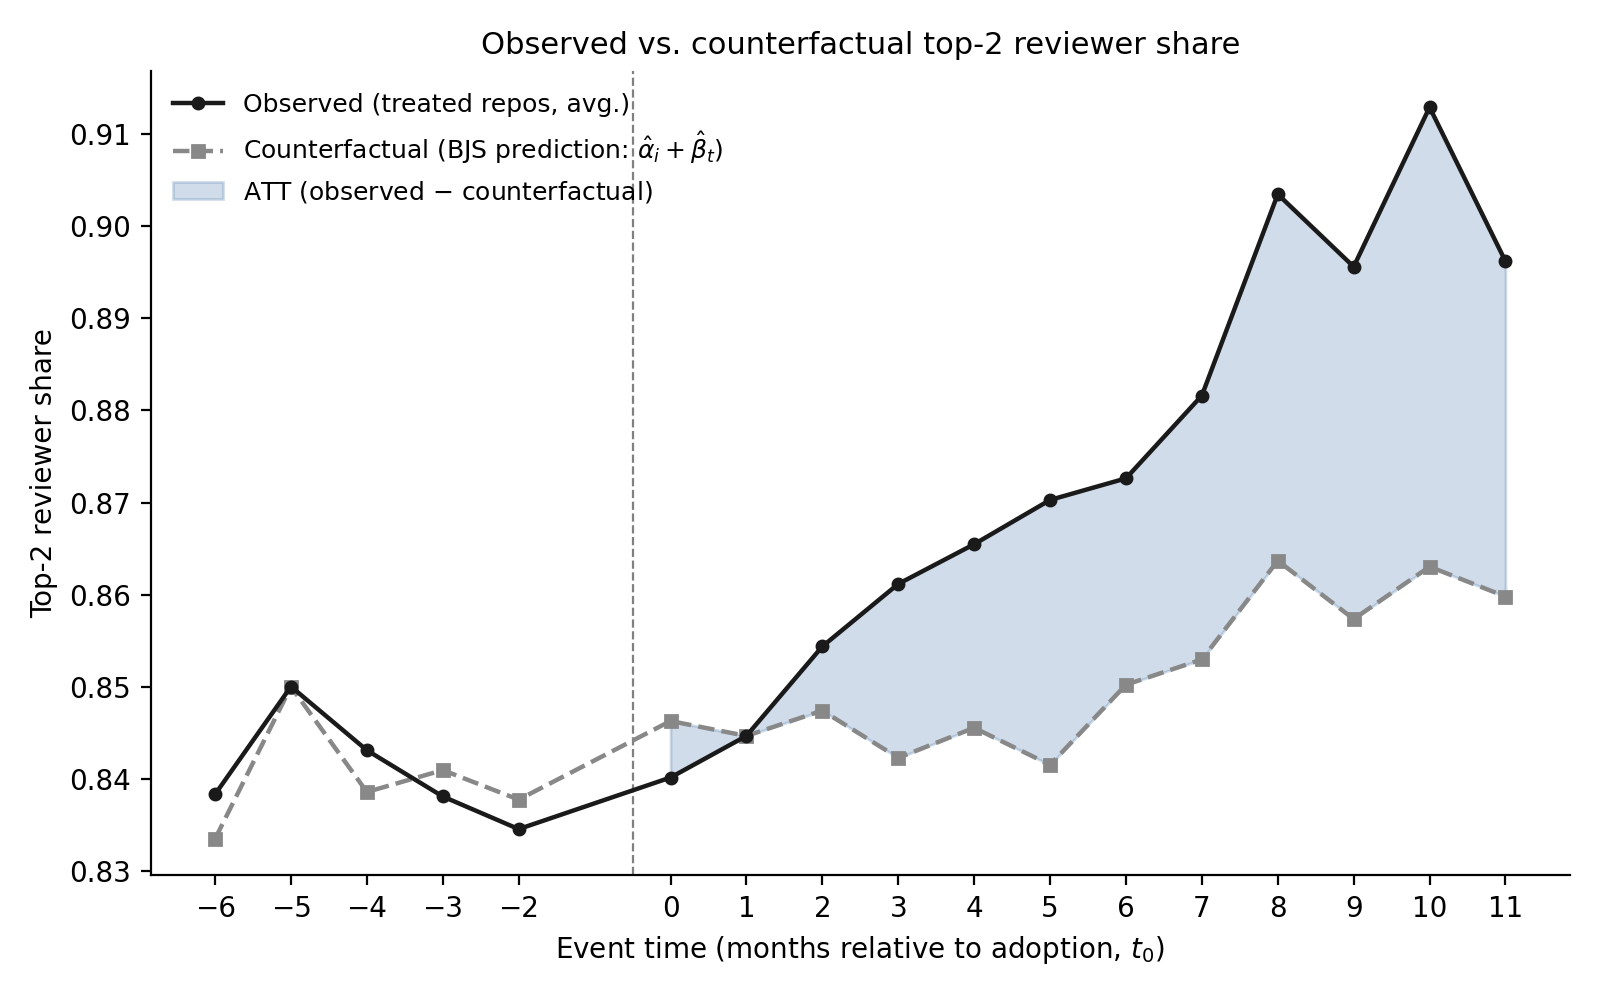
\includegraphics[width=0.85\textwidth]{figures/bjs_illustration_top2_share.png}
\end{center}
\end{frame}

\section{Results}

\begin{frame}{H1 --- Same People, Different Division of Labour}
\begin{table}
\centering
\small
\begin{tabular}{lrr}
\toprule
Outcome & ATT & $p$ \\
\midrule
Top-1 review share & $+0.017$ \ (0.0089) & 0.052 \\
Top-2 review share & $+0.015^{**}$ \ (0.0050) & 0.003 \\
Tail share (outside the top two) & $-0.015^{***}$ & $<0.001$ \\
Reviewer Gini coefficient & $+0.030^{***}$ & $<0.001$ \\
\addlinespace
\multicolumn{3}{l}{\textit{Repos with 3+ reviewers monthly}} \\
Top-1 review share & $+0.041^{***}$ \ (0.0072) & $<0.001$ \\
Top-2 review share & $+0.036^{***}$ \ (0.0052) & $<0.001$ \\
\addlinespace
Repo FE & Yes & \\
Time FE & Yes & \\
\bottomrule
\end{tabular}
\end{table}
\footnotesize All estimates above pass the pre-trend test; team size is unchanged. Gini computed on 1{,}406 of 1{,}771
pairs.
\end{frame}

\begin{frame}{H1 --- What the Numbers Show}
\begin{itemize}
  \item \textbf{Headcount:} team size is unchanged -- the group
        reassigns roles internally, it doesn't grow or shrink.
  \item \textbf{Concentration:} top-2 share rises while tail share
        falls by almost the same amount, and the Gini rises across the
        whole distribution -- work moves up within that fixed group,
        not just between the top two.
  \item Many repo-months start pinned near 100\% (only 1--2 reviewers),
        diluting the pooled estimate; restricting to 3+ reviewers
        roughly doubles it.
\end{itemize}
\vspace{0.3em}
\end{frame}

\begin{frame}{H1 --- Concentration Depends on Whether Leadership Was Already Settled}
Split treated repos by whether one person already held the top spot for
the entire 5-month pre-period (``settled'') or not (``unsettled''):
\begin{table}
\centering
\small
\begin{tabular}{lrr}
\toprule
Outcome & Unsettled leader ($n{=}191$) & Settled leader ($n{=}105$) \\
\midrule
Top-1 review share & $+0.047$ (4.62) & $-0.022$ ($-1.84$) \\
Top-2 review share & $+0.036$ (4.40) & $+0.001$ (0.14) \\
\bottomrule
\end{tabular}
\end{table}
\begin{itemize}
  \item Both strata pass pre-trend cleanly; the difference between them
        is strongly significant (top-1: $p<0.0001$, top-2: $p=0.003$).
  \item \textbf{Caveat:} tenure correlates with pre-adoption
        concentration level ($r=0.38$) -- the same confound flagged for
        the separate concentration-level split. Cannot yet separate a
        genuine threshold effect from mean reversion.
  \item \textbf{Scope:} this subsample (complete 5-month pre-period
        coverage) also skews busier than average ($\sim$2$\times$ the
        pre-period PR volume) -- a real subset, not the general
        population.
\end{itemize}
\end{frame}

\begin{frame}{H2 --- Reassigned, Not Destabilized}
\begin{table}
\centering
\small
\begin{tabular}{lrr}
\toprule
Outcome & ATT & $p$ \\
\midrule
Monthly leader is the pre-adoption top-1 & $-0.077^{***}$ \ (0.0151) & $<0.001$ \\
Monthly top-2 overlaps the pre-adoption top-2 & $-0.045^{***}$ \ (0.0101) & $<0.001$ \\
Month-to-month leader change & $-0.058^{**}$ \ (0.0197) & 0.004 \\
\addlinespace
Repo FE & Yes & \\
Time FE & Yes & \\
\bottomrule
\end{tabular}
\end{table}
\begin{itemize}
  \item The lead shifts to someone new relative to who led before
        adoption -- the shift builds gradually, not at once.
  \item Once that shift happens, it holds: month-to-month leader
        changes become \textbf{less} likely, not more -- one
        reassignment, then stability.
  \item \textbf{Caveat:} the first row is the robust driver of this
        result (survives and strengthens on the control-independence
        check, backup). The month-to-month row does not -- treat it as
        suggestive, not established.
\end{itemize}
\end{frame}

\begin{frame}{Is That Reassignment a Construction Artifact?}
The fixed identity is chosen by taking the maximum over
$h=-6,\dots,-2$, and those same months form the estimation baseline ---
which inflates pre-period persistence by construction.
\begin{center}
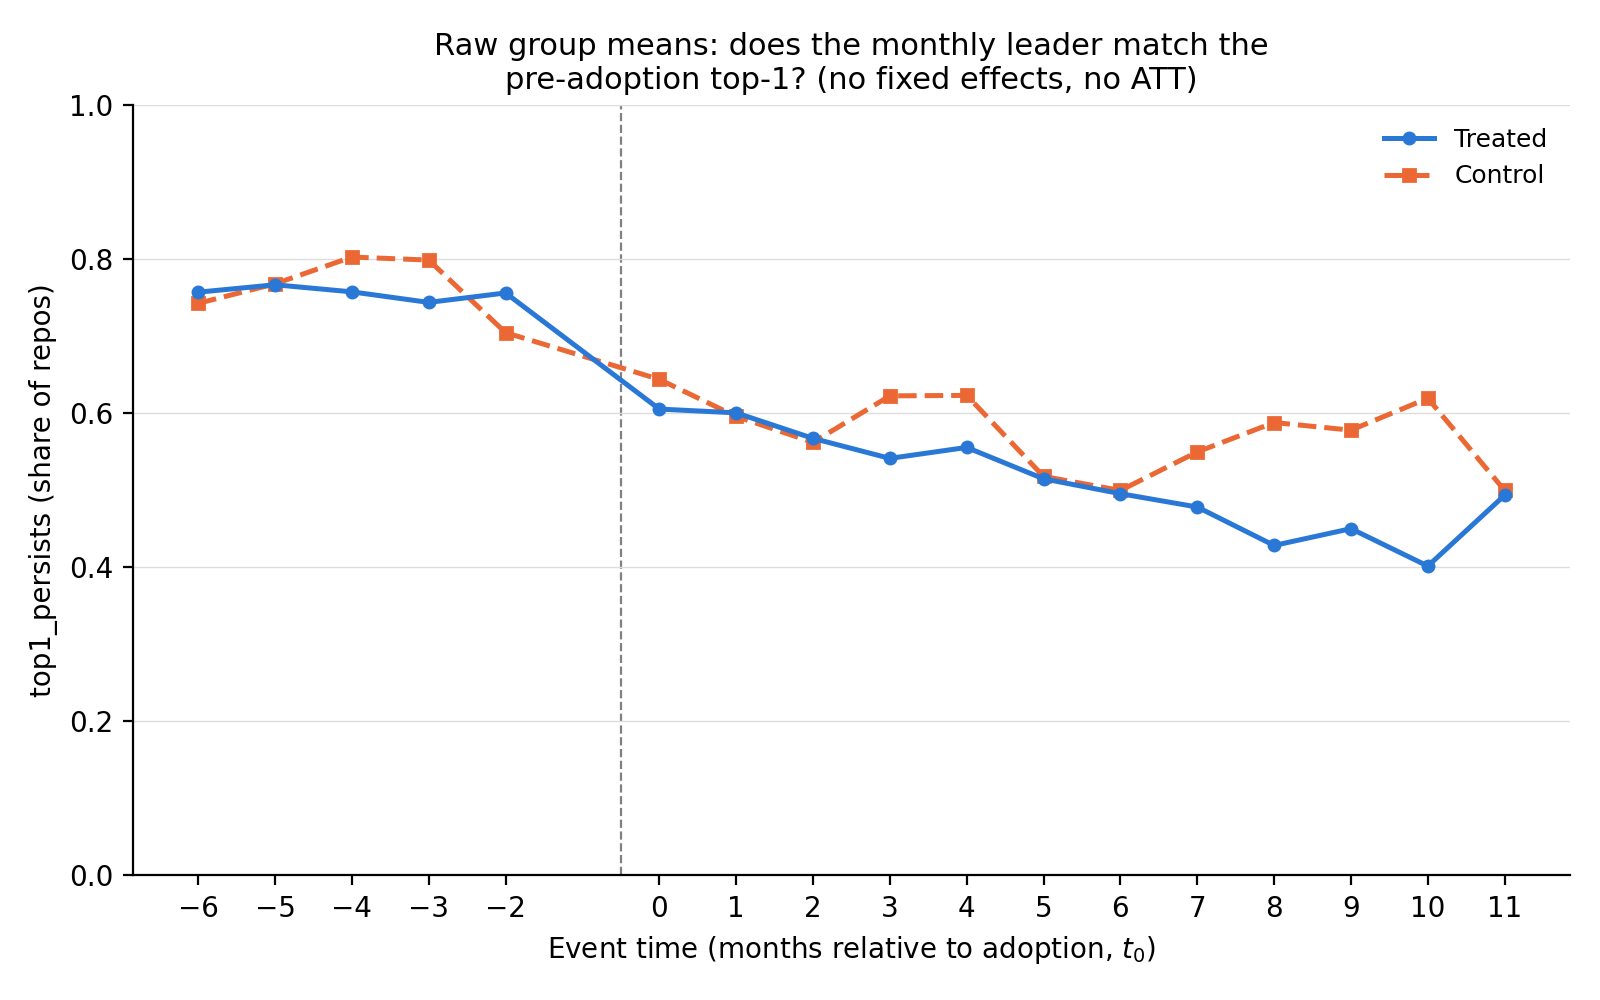
\includegraphics[width=0.72\textwidth]{figures/top1_persists_raw_event_time.png}
\end{center}
\vspace{-0.3em}
\footnotesize Both groups drop from $\sim$0.75 to $\sim$0.60 at
$h\!=\!0$: the artifact is real, and it is common to treated and
control, so the difference-in-differences nets it out. The treated
series separates only later.
\end{frame}

\begin{frame}{H3 --- The Process Signature}
\begin{table}
\centering
\small
\begin{tabular}{lrr}
\toprule
Outcome & ATT & $p$ \\
\midrule
Time to first review (h) & $-65.0^{*}$ \ (28.91) & 0.025 \\
Time to merge (h)        & $-62.8^{*}$ \ (27.10) & 0.021 \\
Review rounds/PR         & $+0.180^{*}$ \ (0.082) & 0.027 \\
\addlinespace
Repo FE & Yes & \\
Time FE & Yes & \\
\bottomrule
\end{tabular}
\end{table}
\begin{itemize}
  \item PRs reach review and merge sooner, but take more rounds to get
        there.
  \item Consistent with verification by someone carrying less
        project history: available sooner, needing more exchange to
        converge.
\end{itemize}
\end{frame}

\begin{frame}{H3 --- Do Pull Requests Just Get Smaller?}
\begin{table}
\centering
\small
\begin{tabular}{lrr}
\toprule
Spec & ATT (hours) & $t$ \\
\midrule
Unrestricted (uncapped PR-level data) & $-34.2$ & $-1.74$ \\
Residualized on PR size & $-35.8$ & $-1.82$ \\
Restricted to similarly-sized PRs (25th--75th pct.) & $-61.8$ & $-2.62$ \\
\bottomrule
\end{tabular}
\end{table}
\begin{itemize}
  \item With PR size held fixed, latency still falls --- merges get
        faster, not merely smaller.
\end{itemize}
\end{frame}

\begin{frame}{H3 --- Reverses in Busy Repos}
On the busier-than-average subsample ($\sim$2$\times$ pre-period PR
volume, $n{=}296$):
\begin{table}
\centering
\small
\begin{tabular}{lrr}
\toprule
Outcome & Full sample & Busy subsample \\
\midrule
Time to merge (h) & $-62.8$ (2.60) & $+40.7$ (2.83) \\
Review rounds/PR & $+0.180$ (4.04) & $-0.146$ (2.04) \\
\bottomrule
\end{tabular}
\end{table}
\begin{itemize}
  \item Both directions pass pre-trend, in both samples -- not a
        construction artifact. Checked and ruled out: $t_0$-timing
        bias, horizon-weighting (the full sample's own $\text{ATT}_h$
        never flips sign across any single horizon).
  \item In high-volume repos, merging gets \textbf{slower} and needs
        \textbf{fewer} rounds after adoption -- the opposite pattern
        from the general sample.
  \item Second independent signal (after H1's stronger-in-big-repos
        result) that large/busy projects respond qualitatively
        differently to AI adoption, not just more intensely.
\end{itemize}
\end{frame}

\section{Discussion}

\begin{frame}{What Changes When AI Arrives}
\begin{enumerate}
  \item \textbf{Same room, different seat}: headcount is unchanged;
        work moves from the periphery to the top.
  \item \textbf{The entry is reassigned, and it holds}: increasingly
        not the pre-adoption lead, widening gradually -- yet not more
        volatile, a rewritten directory.
  \item \textbf{Same signature in the process}: PRs reach review and
        merge sooner but take more rounds to converge.
\end{enumerate}
\vspace{0.4em}
A project's transactive memory can be reassigned by a tooling shock in
a matter of months, with membership constant --- and no throughput,
latency or participation metric registers it.
\end{frame}

\begin{frame}{The Traditional Model: Authority From Memory}
Code review has always run on one assumption: \textbf{the right
reviewer is whoever has accumulated the most memory of this specific
code.} This isn't folklore -- it's how the field has measured and
automated reviewer selection for over a decade.
\begin{itemize}
  \item Review's central function is building shared
        \emph{understanding} of the change, not just catching bugs
        \cite{bacchelli2013expectations}.
  \item State-of-the-art reviewer-recommendation tools formalize this
        directly: recommend whoever has reviewed similar file paths
        before \cite{thongtanunam2015revfinder}, or whoever has the
        deepest historical contribution to the changed files
        \cite{zanjani2016chrev}.
  \item Open-source peer review itself grew up as an informal,
        tenure-based norm -- whoever has been around long enough earns
        the authority to gate changes \cite{rigby2008apache}.
\end{itemize}
\vspace{0.3em}
The reviewer \emph{is} a gatekeeper \cite{allen1977gatekeepers} --
authority is durable, personal, and earned through years of
accumulated exposure to the codebase.
\end{frame}

\begin{frame}{Is That Model Breaking?}
Our own results, read together, say yes -- and we can be precise about
\emph{how}.
\begin{itemize}
  \item \textbf{Durable authority is dissolving into rotation.} A
        reviewer who led one half of the post-adoption window is no
        more likely to still lead the second half, treated vs.\
        control -- concentration is real, but it doesn't settle onto
        fixed individuals the way the traditional model predicts.
  \item \textbf{Suggestive, not yet established: a lower entry
        threshold.} Reassignment is strongest where tenure hadn't
        accumulated, weakest where a leader was already settled -- but
        this correlates (r=0.38) with those same repos' pre-adoption
        concentration level, a confound already flagged elsewhere.
        Can't yet separate a real threshold effect from mean reversion.
  \item \textbf{The apprenticeship pipeline that used to manufacture
        gatekeepers is thinning.} Peripheral, occasional reviewers --
        traditionally how someone earns the file-history that
        REVFINDER-style tools reward -- hold a shrinking share of
        activity.
\end{itemize}
\vspace{0.3em}
Put together: authority is shifting from \emph{accumulated, durable,
personal} to \emph{transient and capacity-based} -- whoever has
bandwidth this month, not whoever has the longest memory.
\end{frame}

\begin{frame}{Reconstructing the Process}
The standard pipeline (earlier slide) treats verification as a
discrete gate at the end: write, then check. That shape assumes
writing is the slow, scarce step.
\begin{itemize}
  \item AI inverts the economics: generating code is now nearly free.
        The bottleneck -- and the organizational weight -- moves
        almost entirely onto verification.
  \item A gate sized for the old economics cannot absorb that weight
        by staying a gate. Our data shows it isn't: the gate is
        already dissolving into a rotating, lower-threshold, less
        memory-dependent function.
  \item The traditional fix -- promote someone with years of context
        -- no longer matches how the role is actually being filled.
\end{itemize}
\vspace{0.3em}
\textbf{The reconstruction this implies:} verification has to become a
distributed, continuously-engineered property of the process, not a
checkpoint inherited from whoever has been there longest.
\end{frame}

\begin{frame}{What This Means in Practice}
\begin{itemize}
  \item \textbf{Stop indexing review capability by tenure.} If
        standing no longer takes years to earn, gatekeeping rules
        built around seniority (file ownership, CODEOWNERS-by-tenure)
        are already out of step with who is actually doing the work.
  \item \textbf{Track participation breadth, not just throughput.} A
        shrinking periphery is an early-warning signal -- like
        bus-factor -- invisible to every speed metric this paper also
        confirms is improving.
  \item \textbf{Engineer the apprenticeship pipeline deliberately.} It
        no longer forms for free; deliberate review-rotation for newer
        contributors has to replace what used to emerge organically.
  \item \textbf{Treat succession as a tracked risk, not an accident.}
        The handover already happens, usually without anyone planning
        it -- the open question is whether it happens \emph{to} a
        system designed for it.
\end{itemize}
\end{frame}

\begin{frame}{Are Our Controls Actually Independent?}
\textbf{Problem:} 37.7\% of repos share a human reviewer with some
treated repo elsewhere in the sample -- that reviewer can carry
AI-adoption habits into a repo we're counting as an untreated
``control,'' violating the no-interference assumption the design needs.
\vspace{0.3em}

\textbf{What we did:} identified the 176 fully independent (``clean'')
pairs and re-ran every headline outcome restricted to them.
\vspace{0.3em}

\textbf{Result if contamination is removed:}
\begin{itemize}
  \item \textbf{Survives and strengthens:} top-2 share, tail share,
        top1\_persists -- the paper's three most load-bearing results.
  \item \textbf{Weakens but same sign:} top-1 share, Gini, time-to-
        merge, review-rounds -- plausibly just power loss at $n{=}176$.
  \item \textbf{Does not survive:} month-to-month leader-change rate --
        collapses to $t{\approx}0$, dropped as a robust claim.
\end{itemize}
\end{frame}

\begin{frame}{Does It Matter Which AI Tool or Era?}
Tested two ways: \textbf{calendar-time adoption era} (proxy for tool
generation, since our signal can't identify model versions) and
\textbf{specific tool identity} (Codex, Copilot, Claude, Cursor).
\vspace{0.3em}
\begin{itemize}
  \item Neither split produces a significant difference in the
        concentration effect -- and that null survives the full
        battery: caliper sensitivity, bootstrap SE, and the clean-
        sample restriction above.
  \item One exception: Codex's own latency effect is individually
        robust (survives all three checks) -- but not provably larger
        than Copilot's or Claude's.
\end{itemize}
\vspace{0.3em}
\textbf{Reading:} the effect is general, not an artifact of any one
tool or AI generation -- a robustness result, not a new mechanism.
\end{frame}

\begin{frame}{Limitations}
\begin{itemize}
  \item \textbf{No downstream outcome}: We measure how verification is
        organized, not what it catches. Nothing here speaks to code
        quality, defects, or security.
  \item \textbf{Detection, not adoption}: $t_0$ is the first
        \emph{observed} signal; controls are never-detected rather than
        never-treated.
  \item \textbf{Merged PRs only}: What is never reviewed or never
        merged is outside the pipeline.
  \item \textbf{Entrant/incumbent share unusable}: The activity-level
        version fails the pre-trend test under the current 6-month
        pre-window definition, so we cannot yet say whether the
        reassigned lead is a long-standing member or a recent one.
  \item \textbf{Distinct-leaders-per-6-months not estimable}: the
        pre-period window (5 months) can never hold a full 6-month
        lookback, so no treated repo contributes pre-period data for
        this specific measure under the current design.
  \item \textbf{Gini not on the complete sample}: 1,406 of 1,771 pairs;
        the remaining 365 lack usable pre+post coverage in the
        repo-month cache, not a Gini-specific gap.
  \item \textbf{Controls are not fully independent}: a meaningful share
        of control repos share a reviewer with some treated repo, and
        this is worse precisely where the effect is strongest (backup).
\end{itemize}
\end{frame}

\begin{frame}{Future Work}
\begin{itemize}
  \item Redefine incumbency over full repository history (needs data
        before $h=-6$, a new extraction) and re-estimate the
        entrant/incumbent split -- the one measure that would close the
        ``who takes over'' question directly.
  \item Attach one downstream outcome (revert rate, post-merge defects,
        contributor retention) to connect structure to consequence --
        needs data types not currently collected.
\end{itemize}
\end{frame}

\begin{frame}[plain]
\begin{center}
\Large Thank you
\vspace{1em}

\normalsize Questions?
\end{center}
\end{frame}

\section{Backup}

\begin{frame}{Outcome Variables: Calculation Detail}
\textbf{top1\_share / top2\_share / tail\_share}: For each repo-month:
\begin{itemize}
  \item Count the distinct merged PRs reviewed by each human reviewer;
        each reviewer counted once per PR regardless of how many review
        events they submitted.
  \item Rank reviewers by this count. top1 is the highest individual
        count; top2 the combined count of the two highest; the tail is
        everyone else. Shares use the sum of all reviewers' counts as
        denominator.
\end{itemize}
\textbf{top1\_persists}: Freeze one identity per repository from the
pre-period only ($h=-6,\dots,-2$): the reviewer with the highest total
across those months. For every month, compare that fixed identity with
that month's busiest reviewer. Note this is a \emph{single person},
distinct from the monthly re-ranking used by top1\_share.
\vspace{0.3em}
\textbf{Reviewer Gini}: Per-PR reviewer identities reconstruct each
repo-month's complete reviewer-count distribution; the Gini of that
distribution (0 = equal split, 1 = one reviewer does everything)
replaces the earlier HHI approximation ($p=0.095$).
\end{frame}

\begin{frame}{Validating an Estimate Before Reporting It}
\begin{itemize}
  \item Parallel-trends check on the pre-period leads (next slide).
  \item Re-estimation at 5 matching calipers (0.10--0.50 SD). Tighter =
        fewer, closer-matched pairs; looser = more pairs, less precise
        matches. Caliper stability = does the result hold at every
        threshold, not just our main choice (0.25)?
  \item Balanced-panel restriction and a fixed 6-month common-horizon
        re-estimate (vs.\ the full 0--11 month window).
  \item Mean-reversion / selection-on-timing diagnostic.
  \item Repo-cluster bootstrap of the BJS standard errors.
  \item Adoption-signal precision re-check on newly collected data.
\end{itemize}
\vspace{0.5em}
An estimate that fails the pre-trend test is excluded from causal
interpretation, whatever its own significance. Two measures were
excluded this way: entrant share and total review count.
\end{frame}

\begin{frame}{Is the Reported Inference Trustworthy?}
Analytic cluster-robust SE vs.\ a 300-replicate repo-pair bootstrap:
\begin{table}
\centering
\scriptsize
\begin{tabular}{lrrrr}
\toprule
Outcome & Analytic SE & Bootstrap SE & Ratio & Corrected $p$ \\
\midrule
Top-1 review share     & 0.0064 & 0.0089 & 1.39$\times$ & 0.052 \\
Top-2 review share     & 0.0034 & 0.0050 & 1.45$\times$ & 0.003 \\
Time to first review   & 21.40  & 28.91  & 1.35$\times$ & 0.025 \\
Time to merge          & 24.18  & 27.10  & 1.12$\times$ & 0.021 \\
Review rounds          & 0.045  & 0.082  & 1.83$\times$ & 0.027 \\
\bottomrule
\end{tabular}
\end{table}
The analytic SE understates true uncertainty by 12--83\%. Top-1 share
drops to borderline ($p=0.052$); everything else survives. All tables
in this deck use the corrected $p$.
\end{frame}

\begin{frame}{The Parallel-Trends Assumption for BJS}
\begin{itemize}
  \item BJS builds each treated repo's counterfactual,
        $\hat\alpha_i+\hat\beta_t$, from a model fit only on
        pre-adoption and control data. That counterfactual is valid
        only if, absent treatment, the repo would have kept following
        that same repo-baseline-plus-calendar-trend path.
  \item Primary check (go/no-go): joint Wald test on the five
        pre-period lead coefficients ($h=-6,\dots,-2$), $\chi^2_5$.
  \item Secondary check (margin of safety): how large an undetected
        pre-trend would need to be, extrapolated forward, to explain
        away the post-period effect --- in units of the estimated
        pre-trend's own SE.
\end{itemize}
\begin{table}
\centering
\scriptsize
\begin{tabular}{lr}
\toprule
Outcome & Breakdown slope, in SE units \\
\midrule
Top-1 review share     & 2.6$\times$ (wrong-signed pre-trend --- helps us) \\
Top-2 review share     & 3.4$\times$ (wrong-signed pre-trend --- helps us) \\
Time to first review   & 3.7$\times$ (same-signed --- erodes $\sim$36\% of ATT) \\
Time to merge          & 3.8$\times$ \\
Review rounds          & 3.0$\times$ (same-signed --- erodes $\sim$55\% of ATT) \\
\bottomrule
\end{tabular}
\end{table}
\end{frame}

\begin{frame}{Robustness Check}
\begin{table}
\centering
\scriptsize
\begin{tabular}{lll}
\toprule
Outcome & Caliper stability (5 tested) & Mean-reversion \\
\midrule
Top-1 review share     & Stable, all 5 calipers & No concern \\
Top-2 review share     & Stable, all 5 (fails pre-trend at 1) & No concern \\
Time to first review   & Stable, all 5 calipers & Mild caveat \\
Time to merge          & Stable, all 5 calipers & Caveat (asymmetry) \\
Review rounds          & Stable 5/5, sig.\ 4/5 (fails pre-trend at 1) & No concern \\
\bottomrule
\end{tabular}
\end{table}
\vspace{0.5em}
\scriptsize No outcome above changes sign at any caliper. Outcomes that
failed validation (raw top-1 review count, entrant share, total review
count) are excluded from causal interpretation.
\end{frame}

\begin{frame}{Is the Full-Window Effect a Cohort Artifact?}
Treated observations shrink from 1,405 at $h{=}0$ to 205 at $h{=}11$ ---
later horizons rest on a smaller, longer-surviving subset of repos.
\begin{table}
\centering
\scriptsize
\begin{tabular}{lrr}
\toprule
Outcome & Full ATT & Common-horizon ATT ($h=0..5$) \\
\midrule
Top-1 review share     & $+0.0173$ & $+0.0075$ \\
Top-2 review share     & $+0.0151$ & $+0.0081$ \\
Time to first review   & $-65.0$   & $-53.1$ \\
Time to merge          & $-62.8$   & $-56.9$ \\
Review rounds          & $+0.180$  & $+0.177$ \\
\bottomrule
\end{tabular}
\end{table}
Concentration's full-window ATT is roughly double the common-horizon
estimate --- part of the apparent late-horizon growth is cohort
composition, not pure treatment dynamics. Since the reassignment effect
in H2 also grows with horizon, the same check is owed for
top1\_persists.
\end{frame}

\begin{frame}{Caveat: A Sampling Cap in the Repo-Month Extraction}
\begin{itemize}
  \item The original repo-month pipeline capped each repo-month at 40
        sampled merged PRs (binds for $\sim$11\% of repo-months). The
        new PR-level extraction has no such cap.
  \item Re-estimating H1 on the identical 802-repo subsample:
\end{itemize}
\begin{table}
\centering
\small
\begin{tabular}{lrr}
\toprule
Outcome & Capped ATT ($t$) & Uncapped ATT ($t$) \\
\midrule
Top-1 review share & $+0.0141$ (2.07) & $+0.0070$ (1.12) \\
Top-2 review share & $+0.0153$ (4.08) & $+0.0082$ (2.47) \\
\bottomrule
\end{tabular}
\end{table}
\begin{itemize}
  \item The cap roughly \textbf{doubles} the concentration point
        estimates where it binds --- top-1 share loses significance
        uncapped, top-2 share survives ($t=2.47$).
  \item Direction is not overturned; the full-sample effect size is
        probably somewhat inflated.
\end{itemize}
\end{frame}

\begin{frame}{Caveat: Controls Are Not Fully Independent}
\begin{itemize}
  \item 37.7\% of repos share a reviewer with some treated repo
        elsewhere in the sample (identity-covered subsample, 309 pairs)
        -- a SUTVA violation. Over half of contaminated repos are
        contaminated via their own \emph{lead} reviewer, not a
        peripheral one.
  \item This is a popular-project effect, not a small-project one:
        contaminated repos have 2$\times$ the reviewer pool of clean
        repos (median 10 vs.\ 5) and more stars/contributors.
\end{itemize}
\begin{table}
\centering
\small
\begin{tabular}{lrr}
\toprule
Outcome & Contaminated-only ($t$) & Clean-only ($t$) \\
\midrule
Top-1 review share & $+0.0376$ (2.46) & $+0.0118$ (0.86) \\
Top-2 review share & $+0.0462$ (4.77) & $+0.0208$ (2.79) \\
\bottomrule
\end{tabular}
\end{table}
\begin{itemize}
  \item The effect is \textbf{stronger}, not weaker, in the
        contaminated segment -- consistent with the 3+-reviewer
        subgroup result, but it means the strongest part of the signal
        sits exactly where control independence is most in question.
  \item Cannot yet separate a genuinely larger effect in bigger/more-
        interconnected projects from inflation due to non-independent
        controls there.
\end{itemize}
\end{frame}

\begin{frame}{Does the Effect Differ by Adoption Era?}
Repos adopted 2025-05 to 2025-11 (``Era 2'', $n{=}413$) vs.\
2025-11 to 2026-05 (``Era 3'', $n{=}666$) -- the two best-powered
calendar-time cohorts, roughly bracketing successive generations of
agentic coding tools:
\begin{table}
\centering
\small
\begin{tabular}{lrrl}
\toprule
Outcome & Era 2 ATT & Era 3 ATT & Diff.\ test \\
\midrule
Top-1 review share & $+0.028$ & $+0.020$ & $p=0.60$ \\
Top-2 review share & $+0.021$ & $+0.014$ & $p=0.42$ \\
\bottomrule
\end{tabular}
\end{table}
\begin{itemize}
  \item No test in a full battery -- caliper sensitivity, bootstrap
        SE, clean-sample restriction -- ever produces a significant
        Era-2-vs-Era-3 difference on this comparison.
  \item \textbf{The effect is not detectably different across adoption
        eras.} Not driven by a specific generation of AI coding tools.
\end{itemize}
\end{frame}

\begin{frame}{Caveat: Era-Specific Estimates Are Individually Fragile}
Same robustness battery applied to each era's own ATT, not just the
Era-2-vs-Era-3 comparison:
\begin{itemize}
  \item \textbf{Caliper:} only 2 of 4 era$\times$outcome cells are
        sign-stable across all 5 calipers -- and Era 2's stable
        outcome isn't the same as Era 3's.
  \item \textbf{Bootstrap (300 reps, within era):} knocks out 3 of 4
        originally-significant cells; only Era 2's top-2 share
        survives ($t=2.12$, $p=0.034$).
  \item \textbf{Clean sample:} none of the 4 cells survive (small
        cells, $n{=}49$/$78$).
\end{itemize}
\vspace{0.3em}
Read carefully: this does \textbf{not} contradict the no-era-difference
finding above -- both eras lose significance under the same pressures,
roughly equally, which is itself consistent with ``no era-specific
effect.'' But splitting into era cohorts should not be cited as two
independently robust confirmations of the headline result; it mostly
reduces $n$ and reproduces known fragility (contamination sensitivity,
caliper sensitivity) already documented elsewhere in this deck.
\end{frame}

\begin{frame}{Does the Effect Differ by Specific Tool?}
Beyond agent-vs-assisted MODE (earlier slide): does it matter whether a
repo adopted Codex, Copilot, Claude, or Cursor specifically? Buckets are
non-exclusive (a repo can carry signals for more than one tool).
\begin{table}
\centering
\small
\begin{tabular}{lrrr}
\toprule
Tool ($n$) & Top-2 share $t$ & Time-to-merge $t$ \\
\midrule
Codex (961)    & $+1.57$ & $-2.97$ \\
Copilot (800)  & $+3.18$ & $-2.60$ \\
Claude (478)   & $+2.55$ & $-1.26$ \\
Cursor (151)   & $+0.66$ & $+1.10$ \\
\bottomrule
\end{tabular}
\end{table}
\begin{itemize}
  \item No pairwise diff-in-ATT among Codex, Copilot, and Claude --
        the three well-powered buckets -- ever reaches significance,
        on either outcome, even after bootstrap correction.
  \item \textbf{No detectable difference by specific tool among the
        buckets with enough power to test.} Consistent with the
        adoption-era finding: the effect is general, not tool-specific.
\end{itemize}
\end{frame}

\begin{frame}{Caveat: Per-Tool Estimates Are Individually Fragile Too}
Same robustness battery applied to each tool's own ATT:
\begin{itemize}
  \item \textbf{Top-2 share: fragile for ALL FOUR tools.} Sign flips
        across the 5 calipers for every single bucket, including
        Copilot and Claude, which looked individually significant at
        the main caliper -- the same matching-artifact signature used
        elsewhere in this deck to reject a result.
  \item \textbf{Time-to-merge is more stable}, and \textbf{Codex's own
        estimate is the one genuinely robust per-tool result here}:
        sign-stable across all 5 calipers, survives bootstrap
        ($t=-2.06$), survives the clean-sample restriction
        ($t=-2.65$, $n{=}85$). Not provably \emph{larger} than
        Copilot's or Claude's effect, though -- just the cleanest on
        its own terms.
  \item Cursor's apparent differences (wrong-signed point estimates,
        the only significant pairwise comparisons) trace to a small,
        caliper-unstable, not-individually-significant bucket -- the
        same ``apparent difference is really just one noisy slice''
        pattern as Era 4's truncated panel, not a real tool effect.
\end{itemize}
\vspace{0.3em}
Read together with the adoption-era result: splitting the pooled
headline findings by any single covariate -- era or tool -- mostly
costs power and reproduces known fragility, rather than revealing a
real source of heterogeneity.
\end{frame}

\begin{frame}{Where Exactly Does the Share Go?}
Full rank-by-rank breakdown (uncapped, full sample) -- not just
top1/top2/tail:
\begin{table}
\centering
\small
\begin{tabular}{lrrr}
\toprule
Rank & ATT & $t$ & Pre-trend \\
\midrule
1 (busiest) & $+0.0066$ & 1.06  & Pass \\
2            & $-0.0078$ & $-1.73$ & Pass \\
3            & $-0.0127^{***}$ & $-4.19$ & Pass \\
4            & $-0.0083^{***}$ & $-3.68$ & Pass \\
5            & $-0.0041^{*}$  & $-2.24$ & Pass \\
\bottomrule
\end{tabular}
\end{table}
\begin{itemize}
  \item Not a clean ``top gains'' story: the single busiest reviewer
        barely moves on this cut. The real, significant losses sit at
        ranks 3--4 -- the moderately-active middle, not the top and
        not just the deep periphery.
  \item Rank 1+2 combined is roughly flat here ($\approx -0.001$) --
        in tension with the capped-pipeline top2\_share headline
        ($+0.015$). A third, independent confirmation of the sampling-
        cap caveat (next slide), not a new separate issue.
  \item Best current read: the moderately-active middle hollows out,
        while the very top holds roughly steady -- a more precise, and
        different, story than ``work piles onto the top two.''
\end{itemize}
\end{frame}

\begin{frame}{Robustness to Control Independence: Full Table}
All 10 headline outcomes, re-estimated on the 176 reviewer-independent
("clean") pairs vs.\ the full sample. All 10 pass pre-trend on the
clean sample -- not a construction artifact.
\begin{table}
\centering
\scriptsize
\begin{tabular}{lrrl}
\toprule
Outcome & Full $t$ & Clean (176) $t$ & Verdict \\
\midrule
Top-1 share            & 1.91  & 0.86  & Weakens \\
Top-2 share             & 3.00  & 2.79  & \textbf{Survives, strengthens} \\
Tail share               & $-3.00$ & $-2.79$ & \textbf{Survives, strengthens} \\
Reviewer Gini            & ---   & 1.49  & Weakens \\
top1\_persists            & $-5.10$ & $-3.70$ & \textbf{Survives, strengthens} \\
top2\_overlap             & $-4.46$ & 0.45  & Null (not a confident reversal) \\
Month-to-month leader change & $-2.95$ & $-0.02$ & \textbf{Collapses} \\
Time to first review     & $-2.25$ & $-2.92$ & Survives, strengthens \\
Time to merge             & $-2.32$ & $-1.88$ & Weakens \\
Review rounds              & 2.20  & 1.82  & Weakens (sign holds) \\
\bottomrule
\end{tabular}
\end{table}
\begin{itemize}
  \item The paper's two most load-bearing rows -- top-2 share and
        top1\_persists -- are also the most robust.
  \item Month-to-month leader change does not survive; drop it from any
        claim of robustness, report top1\_persists as H2's driver.
\end{itemize}
\end{frame}

\begin{frame}{Does the Adoption Mode Matter?}
Agent-authored PRs vs.\ human-committed AI-assisted trailers only,
bootstrap-corrected difference test:
\begin{table}
\centering
\scriptsize
\begin{tabular}{lrrl}
\toprule
Outcome & Agent ATT & Assisted ATT & Difference \\
\midrule
Top-1 share    & $+0.010$ (n.s.) & $+0.039^{*}$    & $p=0.114$ (n.s.) \\
Top-2 share    & $+0.009$ (n.s.) & $+0.033^{***}$  & $p=0.037$ \\
Time to 1st review & $-57.3$ (n.s.) & $-73.6^{*}$  & $p=0.75$ (n.s.) \\
Time to merge  & $-67.2^{*}$     & $-43.4$ (n.s.)  & $p=0.60$ (n.s.) \\
Review rounds  & $+0.24^{*}$     & $-0.01$ (n.s.)  & $p=0.096$ (n.s.) \\
\bottomrule
\end{tabular}
\end{table}
Only the top-2-share difference survives correction ($p=0.037$). We
treat ``adoption mode matters'' as suggestive, not established.
\end{frame}

\begin{frame}{Robustness Check: Does the Result Vary by Team Size?}
Repos split into small-pool and large-pool halves by pre-adoption
reviewer count:
\begin{table}
\centering
\scriptsize
\begin{tabular}{lrrl}
\toprule
Outcome & Small-pool ATT & Large-pool ATT & Diff.\ test \\
\midrule
Time to 1st review & $-53.2$ (n.s., fails pre-trend) & $-80.0$ (n.s.) & $p=0.65$ \\
Time to merge      & $-64.8^{*}$                     & $-56.7$ (n.s.) & $p=0.89$ \\
Review rounds      & $+0.28^{**}$ (fails pre-trend)  & $+0.08$ (n.s.) & $p=0.28$ \\
\bottomrule
\end{tabular}
\end{table}
H3's process results hold whether the starting team was small or large.
One split that looked significant before correction (small pools,
review rounds) disappeared once properly tested.
\end{frame}.
%
% REWRITE NOTES (read before compiling)
% ---------------------------------------------------------------------
% New \cite keys required in the .bib:
%   perry2023users, pearce2022asleep, paradis2025speed,
%   hoffmann2025generative, adams2026radar, gao2026autopilot,
%   zhong2026generations, wegner1987transactive, lewis2003measuring,
%   ren2011transactive
%
% New figure required:
%   figures/top1_persists_raw_event_time.png
%   (raw group means of top1_persists by event time, treated vs control)
%
% Claims deliberately removed because the data does not support them:
%   "fewer hands" / "review lands on fewer people"  -> n_reviewers is null
%   "single point of failure"                       -> top1_persists falls
% =========================================================================

\section{Motivation}

\begin{frame}{AI Boosts Developer Productivity}
\begin{itemize}
  \item RCT evidence: developers using GitHub Copilot completed a
        standardized coding task 55.8\% faster than a control group
        \cite{peng2023impact}.
  \item Enterprise RCT: 96 Google engineers on a complex,
        enterprise-grade C++ task were about 21\% faster with AI
        assistance \cite{paradis2025speed}.
  \item Field and multi-firm evidence points the same way
        \cite{ziegler2022productivity,cui2024effects}.
  \item This is a well-established empirical fact: AI assistance makes
        the authoring of code faster.
\end{itemize}
\end{frame}

\begin{frame}{Verification Problem}
\begin{itemize}
  \item Faster authoring means more code arriving at the review gate,
        while review itself stays human work.
  \item That code is not trustworthy by default. Across 54
        security-relevant scenarios, 44\% of the 1,084 valid programs
        Copilot produced contained a MITRE CWE
        \cite{pearce2022asleep}.
  \item In a controlled user study, participants with an AI assistant
        wrote significantly less secure code than those without --- and
        were likelier to believe their code was secure
        \cite{perry2023users}.
  \item Bird et al.\ (GitHub / Microsoft Research) describe the same
        shift from the inside: effort moves from writing code toward
        verifying it \cite{bird2023taking}.
\end{itemize}
\vspace{0.3em}
Verification is where the work lands and where the risk concentrates.
The question this paper asks is how a project absorbs it.
\end{frame}

\section{Literature Review}

\begin{frame}{Related Work: Team-Level Effects Already Documented}
\begin{itemize}
  \item Review depth rises 5.3\% in a matched staggered-DiD study of
        11,097 repositories \cite{zhang2026augmentation}.
  \item Human reviewers exchange 11.8\% more rounds reviewing
        AI-generated code \cite{zhong2026synergy}.
  \item An enterprise throughput mandate roughly doubles per-reviewer
        load \cite{he2026aiwrites}.
\end{itemize}
\end{frame}

\begin{frame}{Related Work: Team Coordination Specifically}
\begin{itemize}
  \item AI access shifts developer time away from collaborative and
        management tasks toward solo coding, strongest for lower-skill
        developers \cite{hoffmann2025generative}.
  \item At Meta, lines of code per human-landed diff rose 105.9\%
        year-over-year, driven substantially by agentic AI --- review
        demand is outpacing reviewer bandwidth \cite{adams2026radar}.
  \item Governance of AI-assisted contributions varies sharply: many
        AI-co-authored PRs merge with minimal or no human review
        \cite{gao2026autopilot}.
  \item Across 1.02M pull requests, agent-involved review is faster but
        not higher-quality \cite{zhong2026generations}.
\end{itemize}
\end{frame}

\begin{frame}{Related Work: The Gap}
Closest comparator: Copilot adoption raises project-level contributions
5.9\% and coordination time 8\%; core-developer reviews, reviews per
core developer, and distinct core reviewers all rise
\cite{song2026impact}.
\vspace{0.3em}
\textbf{What no one has tested:}
\begin{itemize}
  \item Averages hide division -- ten reviewers each doing slightly more
        looks identical to one doing far more.
  \item Counts are not structure -- more reviewers taking part doesn't
        mean the work is spread across them.
  \item No one asks \emph{which} people the work is assigned to, or
        whether that assignment holds.
\end{itemize}
\end{frame}

\section{Theory}

% \begin{frame}{Review as a Transactive Memory System}
% A transactive memory system (TMS) is a group's shared directory of
% \emph{who knows what} -- members specialize, and the group knows whom
% to route a problem to \cite{wegner1987transactive,lewis2003measuring,ren2011transactive}.
% \begin{itemize}
%   \item In software, that directory is built from accumulated codebase
%         memory: why a decision was made, what broke before.
%   \item Review is where it's exercised -- who reviews what determines
%         what gets caught.
%   \item Open-source review makes it \textbf{observable}: assignment is
%         recorded behaviour, not survey data.
% \end{itemize}
% \vspace{0.3em}
% TMS separates two things the throughput literature conflates: how
% \emph{specialized} verification is, and \emph{whom} it's specialized
% onto.
% \end{frame}

\begin{frame}{Standard Pipeline}
\begin{center}
\includegraphics[width=0.7\textwidth]{figures/code_process.png}
\end{center}
\footnotesize\centering Standard pipeline
\end{frame}

\begin{frame}{The Review Process, Before AI}
\begin{center}
\includegraphics[width=0.78\textwidth]{figures/review_process.png}
\end{center}
\footnotesize\centering Inside ``Code Review''
\\
\vspace{0.5em}
\end{frame}

\begin{frame}{What AI Changes: From Memory to Capacity}
\begin{itemize}
  \item AI substitutes for code creation, not verification -- it
        enlarges verification instead, and that work leans less on
        accumulated project memory (AI code arrives already clean and
        idiomatic).
  \item As the memory-dependent share shrinks, comparative advantage
        moves from whoever holds the deepest history to whoever has
        capacity to process volume.
\end{itemize}
\vspace{0.2em}
\textbf{Prediction:} the directory entry for ``who verifies this
codebase'' gets \emph{reassigned} -- not because the incumbent leaves,
but because what made them the incumbent matters less.
\end{frame}

\begin{frame}{Hypotheses}
\textbf{Research question:} when AI raises the volume of code needing
verification, how does a project's review directory reorganize?
\begin{enumerate}
  \item[H1] Verification concentrates on fewer specialists inside the
        existing team -- headcount stays the same, roles reassign.
  \item[H2] The pre-adoption lead is displaced from the top position,
        and the new arrangement is stable rather than volatile.
  \item[H3] Verification with less historical context reaches PRs
        sooner but needs more rounds to converge.
\end{enumerate}
\end{frame}

\section{Research Design and Data}

\begin{frame}{Research Design}
\begin{itemize}
  \item Treatment: a repository's own AI-tool adoption, $t_0$ =
        earliest detected signal.
  \item Staggered-adoption DiD on covariate-matched treated/control
        repositories.
  \item Imputation estimator of \cite{borusyak2024revisiting} ---
        avoids the ``forbidden comparisons'' bias of naive two-way
        fixed effects under staggered timing
        \cite{goodman2021difference,callaway2021difference}.
  \item 1,771 matched pairs, 20,188 repository-month observations.
\end{itemize}
\end{frame}

\begin{frame}{Data Construction}
\begin{itemize}
  \item 8,972 candidate repositories, stratified across 6 languages
        $\times$ 4 creation-year cohorts, quality-filtered ($\geq$10
        stars, not a fork, minimum contributor count, recent activity
        \cite{munaiah2017curating}).
  \item AI-adoption signal (OR-combined): autonomous agent PR
        authorship, commit co-authorship trailers, configuration-file
        presence. $t_0$ = first detected signal of any kind.
  \item[] 8,972 candidates $\rightarrow$ 2,320 matched pairs (caliper
        0.25 SD) $\rightarrow$ 1,771 pairs with complete panel data.
\end{itemize}
\end{frame}

\begin{frame}{Covariate Balance}
\begin{table}
\centering
\small
\begin{tabular}{lccc}
\toprule
Covariate & Treated & Control & Norm. diff. \\
\midrule
\multicolumn{4}{l}{\textit{Before matching ($n=8{,}972$)}} \\
$\log(\text{stars})$          & 8.499 & 7.800 & 0.635 \\
$\log(\text{contributors}+1)$ & 3.709 & 2.646 & 0.860 \\
\addlinespace
\multicolumn{4}{l}{\textit{After matching ($n=2{,}320$ pairs)}} \\
$\log(\text{stars})$          & --- & --- & 0.072 \\
$\log(\text{contributors}+1)$ & --- & --- & 0.015 \\
\bottomrule
\end{tabular}
\end{table}
\end{frame}

\begin{frame}{Outcome Variables}
Each measured per repository-month; construction detail in backup.
\begin{itemize}
  \item \textbf{Specialization:} top1\_share/top2\_share -- the busiest
        one/two reviewers' share of a repo-month's total human review
        activity; tail\_share is the complement held by everyone else.
  \item \textbf{Directory assignment:} top1\_persists: is this month's
        busiest reviewer the same person as the repository's fixed
        pre-period top-1? Same for the top-2 pair.
\end{itemize}
\end{frame}

\begin{frame}{Outcome Variables}
Gini coefficient over a repo-month's full reviews-per-reviewer
distribution: 
\[
G = \frac{\sum_{i=1}^{n}\sum_{j=1}^{n} |x_i - x_j|}{2n\sum_{i=1}^{n} x_i}
\]
\begin{itemize}
  \item $x_i$ = number of reviews reviewer $i$ submitted that
        repo-month; $n$ = number of distinct human reviewers that
        repo-month.
  \item G = 0 mean every reviewer handled an equal share.
  \item G = 1 mean one reviewer handled all of it.
\end{itemize}
\end{frame}

\section{Empirical Strategy}

\begin{frame}{Introducing BJS: Why We Need It}
\begin{itemize}
  \item Repos adopt AI at different times --- naive two-way fixed
        effects implicitly compares late adopters against
        already-treated early adopters, not just never-treated
        controls.
  \item These ``forbidden comparisons'' bias the estimate whenever the
        treatment effect changes over time
        \cite{goodman2021difference} --- exactly our case, since our
        effects grow across the post-period.
  \item We use the imputation estimator of
        \cite{borusyak2024revisiting} (``BJS''): it builds each treated
        repo's counterfactual only from never-yet-treated data, so an
        already-treated repo can never contaminate another's
        comparison.
\end{itemize}
\end{frame}

\begin{frame}{Estimator}
Two-step imputation \cite{borusyak2024revisiting}:
\begin{enumerate}
  \item Fit $y_{it}=\alpha_i+\beta_t+\varepsilon_{it}$ on $\Omega_0$
        (controls' full history + treated repos' pre-$t_0$
        observations only).
  \item Predict $\hat y_{it}(0)=\hat\alpha_i+\hat\beta_t$ for treated
        post-$t_0$ observations; $\text{ATT}_h$ = mean residual at
        event-time horizon $h$.
\end{enumerate}
\vspace{0.5em}
Event time: pre-leads $h=-6,\dots,-2$ (no-anticipation: $h=-1$
excluded), post-period $h=0,\dots,11$.
\vspace{0.5em}
Post-adoption data = a treated repo's own observations after its $t_0$.
Step 1 never uses it.
\end{frame}

\begin{frame}{BJS in Practice: Observed vs.\ Counterfactual}
\begin{center}
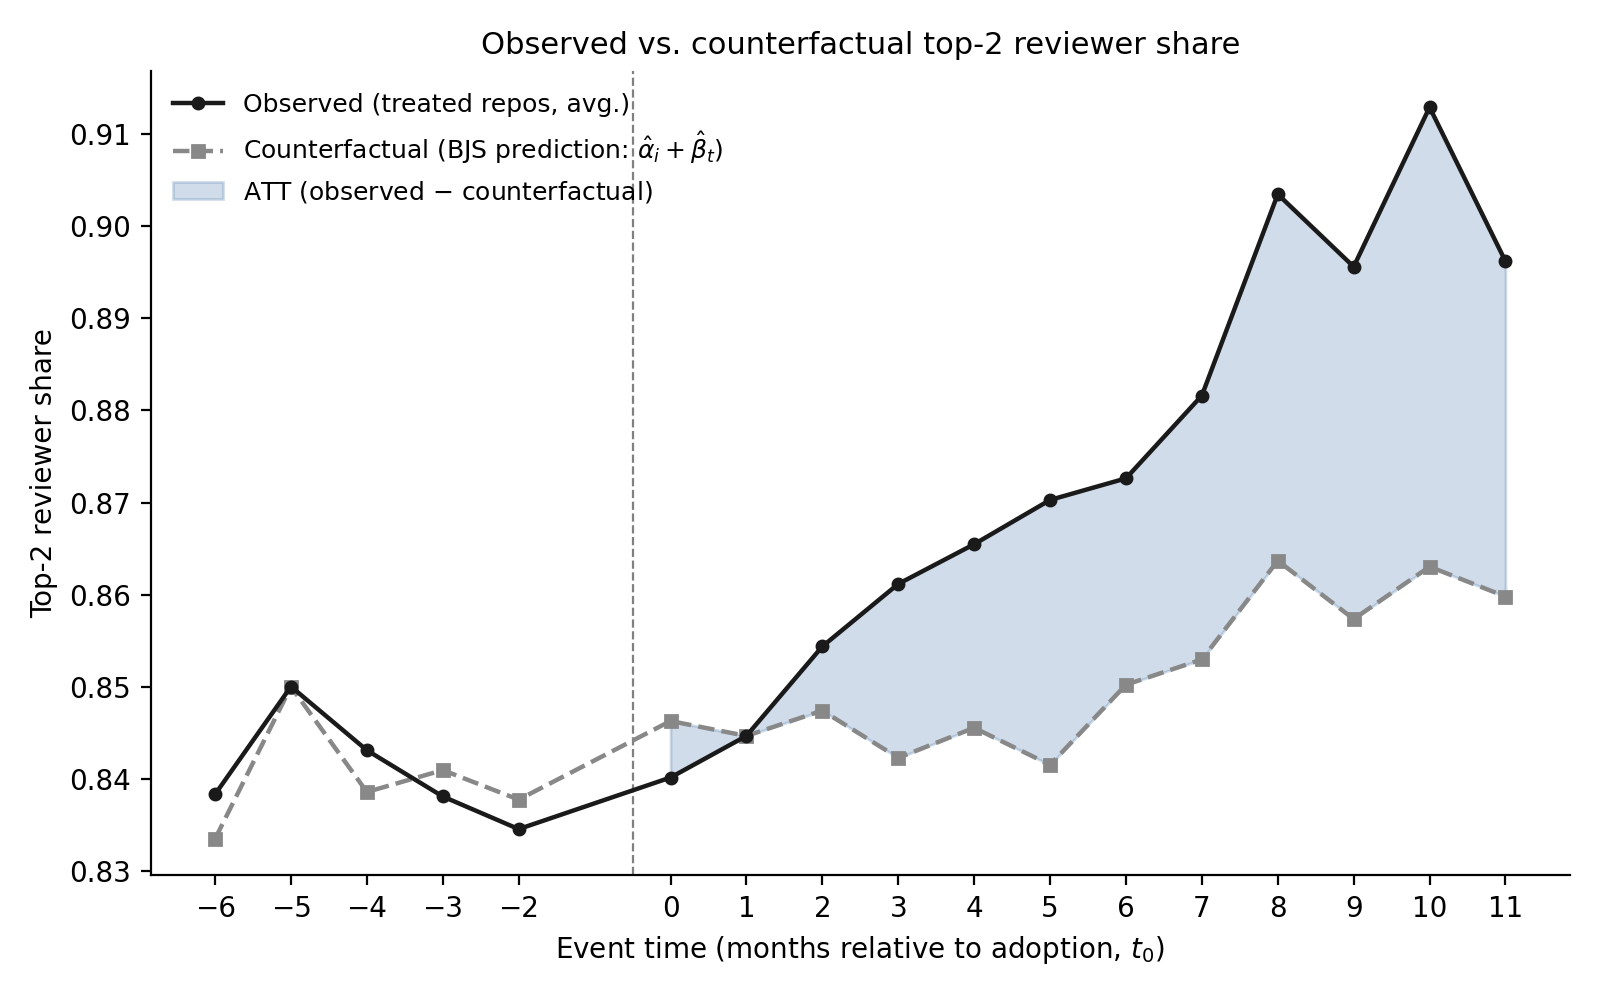
\includegraphics[width=0.85\textwidth]{figures/bjs_illustration_top2_share.png}
\end{center}
\end{frame}

\section{Results}

\begin{frame}{H1 --- Same People, Different Division of Labour}
\begin{table}
\centering
\small
\begin{tabular}{lrr}
\toprule
Outcome & ATT & $p$ \\
\midrule
Top-1 review share & $+0.017$ \ (0.0089) & 0.052 \\
Top-2 review share & $+0.015^{**}$ \ (0.0050) & 0.003 \\
Tail share (outside the top two) & $-0.015^{***}$ & $<0.001$ \\
Reviewer Gini coefficient & $+0.030^{***}$ & $<0.001$ \\
\addlinespace
\multicolumn{3}{l}{\textit{Repos with 3+ reviewers monthly}} \\
Top-1 review share & $+0.041^{***}$ \ (0.0072) & $<0.001$ \\
Top-2 review share & $+0.036^{***}$ \ (0.0052) & $<0.001$ \\
\addlinespace
Repo FE & Yes & \\
Time FE & Yes & \\
\bottomrule
\end{tabular}
\end{table}
\footnotesize All estimates above pass the pre-trend test; team size is unchanged. Gini computed on 1{,}406 of 1{,}771
pairs.
\end{frame}

\begin{frame}{H1 --- What the Numbers Show}
\begin{itemize}
  \item \textbf{Headcount:} team size is unchanged -- the group
        reassigns roles internally, it doesn't grow or shrink.
  \item \textbf{Concentration:} top-2 share rises while tail share
        falls by almost the same amount, and the Gini rises across the
        whole distribution -- work moves up within that fixed group,
        not just between the top two.
  \item Many repo-months start pinned near 100\% (only 1--2 reviewers),
        diluting the pooled estimate; restricting to 3+ reviewers
        roughly doubles it.
\end{itemize}
\vspace{0.3em}
\end{frame}

\begin{frame}{H1 --- Concentration Depends on Whether Leadership Was Already Settled}
Split treated repos by whether one person already held the top spot for
the entire 5-month pre-period (``settled'') or not (``unsettled''):
\begin{table}
\centering
\small
\begin{tabular}{lrr}
\toprule
Outcome & Unsettled leader ($n{=}191$) & Settled leader ($n{=}105$) \\
\midrule
Top-1 review share & $+0.047$ (4.62) & $-0.022$ ($-1.84$) \\
Top-2 review share & $+0.036$ (4.40) & $+0.001$ (0.14) \\
\bottomrule
\end{tabular}
\end{table}
\begin{itemize}
  \item Both strata pass pre-trend cleanly; the difference between them
        is strongly significant (top-1: $p<0.0001$, top-2: $p=0.003$).
  \item \textbf{Caveat:} tenure correlates with pre-adoption
        concentration level ($r=0.38$) -- the same confound flagged for
        the separate concentration-level split. Cannot yet separate a
        genuine threshold effect from mean reversion.
  \item \textbf{Scope:} this subsample (complete 5-month pre-period
        coverage) also skews busier than average ($\sim$2$\times$ the
        pre-period PR volume) -- a real subset, not the general
        population.
\end{itemize}
\end{frame}

\begin{frame}{H2 --- Reassigned, Not Destabilized}
\begin{table}
\centering
\small
\begin{tabular}{lrr}
\toprule
Outcome & ATT & $p$ \\
\midrule
Monthly leader is the pre-adoption top-1 & $-0.077^{***}$ \ (0.0151) & $<0.001$ \\
Monthly top-2 overlaps the pre-adoption top-2 & $-0.045^{***}$ \ (0.0101) & $<0.001$ \\
Month-to-month leader change & $-0.058^{**}$ \ (0.0197) & 0.004 \\
\addlinespace
Repo FE & Yes & \\
Time FE & Yes & \\
\bottomrule
\end{tabular}
\end{table}
\begin{itemize}
  \item The lead shifts to someone new relative to who led before
        adoption -- the shift builds gradually, not at once.
  \item Once that shift happens, it holds: month-to-month leader
        changes become \textbf{less} likely, not more -- one
        reassignment, then stability.
  \item \textbf{Caveat:} the first row is the robust driver of this
        result (survives and strengthens on the control-independence
        check, backup). The month-to-month row does not -- treat it as
        suggestive, not established.
\end{itemize}
\end{frame}

\begin{frame}{Is That Reassignment a Construction Artifact?}
The fixed identity is chosen by taking the maximum over
$h=-6,\dots,-2$, and those same months form the estimation baseline ---
which inflates pre-period persistence by construction.
\begin{center}
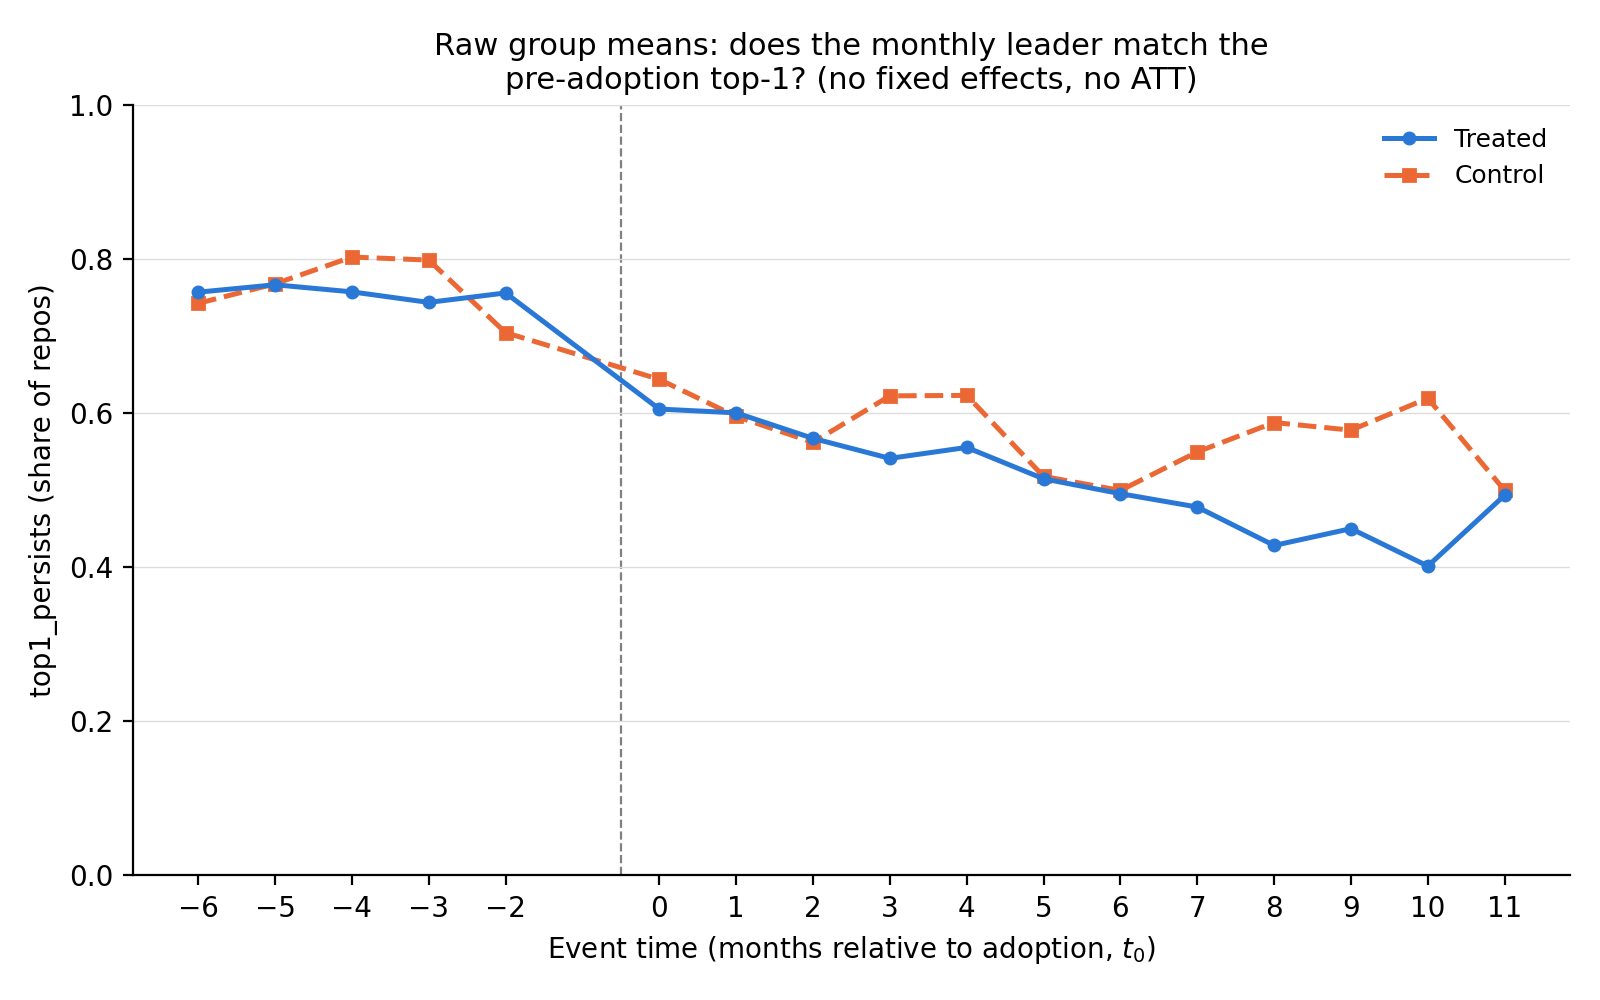
\includegraphics[width=0.72\textwidth]{figures/top1_persists_raw_event_time.png}
\end{center}
\vspace{-0.3em}
\footnotesize Both groups drop from $\sim$0.75 to $\sim$0.60 at
$h\!=\!0$: the artifact is real, and it is common to treated and
control, so the difference-in-differences nets it out. The treated
series separates only later.
\end{frame}

\begin{frame}{H3 --- The Process Signature}
\begin{table}
\centering
\small
\begin{tabular}{lrr}
\toprule
Outcome & ATT & $p$ \\
\midrule
Time to first review (h) & $-65.0^{*}$ \ (28.91) & 0.025 \\
Time to merge (h)        & $-62.8^{*}$ \ (27.10) & 0.021 \\
Review rounds/PR         & $+0.180^{*}$ \ (0.082) & 0.027 \\
\addlinespace
Repo FE & Yes & \\
Time FE & Yes & \\
\bottomrule
\end{tabular}
\end{table}
\begin{itemize}
  \item PRs reach review and merge sooner, but take more rounds to get
        there.
  \item Consistent with verification by someone carrying less
        project history: available sooner, needing more exchange to
        converge.
\end{itemize}
\end{frame}

\begin{frame}{H3 --- Do Pull Requests Just Get Smaller?}
\begin{table}
\centering
\small
\begin{tabular}{lrr}
\toprule
Spec & ATT (hours) & $t$ \\
\midrule
Unrestricted (uncapped PR-level data) & $-34.2$ & $-1.74$ \\
Residualized on PR size & $-35.8$ & $-1.82$ \\
Restricted to similarly-sized PRs (25th--75th pct.) & $-61.8$ & $-2.62$ \\
\bottomrule
\end{tabular}
\end{table}
\begin{itemize}
  \item With PR size held fixed, latency still falls --- merges get
        faster, not merely smaller.
\end{itemize}
\end{frame}

\begin{frame}{H3 --- Reverses in Busy Repos}
On the busier-than-average subsample ($\sim$2$\times$ pre-period PR
volume, $n{=}296$):
\begin{table}
\centering
\small
\begin{tabular}{lrr}
\toprule
Outcome & Full sample & Busy subsample \\
\midrule
Time to merge (h) & $-62.8$ (2.60) & $+40.7$ (2.83) \\
Review rounds/PR & $+0.180$ (4.04) & $-0.146$ (2.04) \\
\bottomrule
\end{tabular}
\end{table}
\begin{itemize}
  \item Both directions pass pre-trend, in both samples -- not a
        construction artifact. Checked and ruled out: $t_0$-timing
        bias, horizon-weighting (the full sample's own $\text{ATT}_h$
        never flips sign across any single horizon).
  \item In high-volume repos, merging gets \textbf{slower} and needs
        \textbf{fewer} rounds after adoption -- the opposite pattern
        from the general sample.
  \item Second independent signal (after H1's stronger-in-big-repos
        result) that large/busy projects respond qualitatively
        differently to AI adoption, not just more intensely.
\end{itemize}
\end{frame}

\section{Discussion}

\begin{frame}{What Changes When AI Arrives}
\begin{enumerate}
  \item \textbf{Same room, different seat}: headcount is unchanged;
        work moves from the periphery to the top.
  \item \textbf{The entry is reassigned, and it holds}: increasingly
        not the pre-adoption lead, widening gradually -- yet not more
        volatile, a rewritten directory.
  \item \textbf{Same signature in the process}: PRs reach review and
        merge sooner but take more rounds to converge.
\end{enumerate}
\vspace{0.4em}
A project's transactive memory can be reassigned by a tooling shock in
a matter of months, with membership constant --- and no throughput,
latency or participation metric registers it.
\end{frame}

\begin{frame}{The Traditional Model: Authority From Memory}
Code review has always run on one assumption: \textbf{the right
reviewer is whoever has accumulated the most memory of this specific
code.} This isn't folklore -- it's how the field has measured and
automated reviewer selection for over a decade.
\begin{itemize}
  \item Review's central function is building shared
        \emph{understanding} of the change, not just catching bugs
        \cite{bacchelli2013expectations}.
  \item State-of-the-art reviewer-recommendation tools formalize this
        directly: recommend whoever has reviewed similar file paths
        before \cite{thongtanunam2015revfinder}, or whoever has the
        deepest historical contribution to the changed files
        \cite{zanjani2016chrev}.
  \item Open-source peer review itself grew up as an informal,
        tenure-based norm -- whoever has been around long enough earns
        the authority to gate changes \cite{rigby2008apache}.
\end{itemize}
\vspace{0.3em}
The reviewer \emph{is} a gatekeeper \cite{allen1977gatekeepers} --
authority is durable, personal, and earned through years of
accumulated exposure to the codebase.
\end{frame}

\begin{frame}{Is That Model Breaking?}
Our own results, read together, say yes -- and we can be precise about
\emph{how}.
\begin{itemize}
  \item \textbf{Durable authority is dissolving into rotation.} A
        reviewer who led one half of the post-adoption window is no
        more likely to still lead the second half, treated vs.\
        control -- concentration is real, but it doesn't settle onto
        fixed individuals the way the traditional model predicts.
  \item \textbf{Suggestive, not yet established: a lower entry
        threshold.} Reassignment is strongest where tenure hadn't
        accumulated, weakest where a leader was already settled -- but
        this correlates (r=0.38) with those same repos' pre-adoption
        concentration level, a confound already flagged elsewhere.
        Can't yet separate a real threshold effect from mean reversion.
  \item \textbf{The apprenticeship pipeline that used to manufacture
        gatekeepers is thinning.} Peripheral, occasional reviewers --
        traditionally how someone earns the file-history that
        REVFINDER-style tools reward -- hold a shrinking share of
        activity.
\end{itemize}
\vspace{0.3em}
Put together: authority is shifting from \emph{accumulated, durable,
personal} to \emph{transient and capacity-based} -- whoever has
bandwidth this month, not whoever has the longest memory.
\end{frame}

\begin{frame}{Reconstructing the Process}
The standard pipeline (earlier slide) treats verification as a
discrete gate at the end: write, then check. That shape assumes
writing is the slow, scarce step.
\begin{itemize}
  \item AI inverts the economics: generating code is now nearly free.
        The bottleneck -- and the organizational weight -- moves
        almost entirely onto verification.
  \item A gate sized for the old economics cannot absorb that weight
        by staying a gate. Our data shows it isn't: the gate is
        already dissolving into a rotating, lower-threshold, less
        memory-dependent function.
  \item The traditional fix -- promote someone with years of context
        -- no longer matches how the role is actually being filled.
\end{itemize}
\vspace{0.3em}
\textbf{The reconstruction this implies:} verification has to become a
distributed, continuously-engineered property of the process, not a
checkpoint inherited from whoever has been there longest.
\end{frame}

\begin{frame}{What This Means in Practice}
\begin{itemize}
  \item \textbf{Stop indexing review capability by tenure.} If
        standing no longer takes years to earn, gatekeeping rules
        built around seniority (file ownership, CODEOWNERS-by-tenure)
        are already out of step with who is actually doing the work.
  \item \textbf{Track participation breadth, not just throughput.} A
        shrinking periphery is an early-warning signal -- like
        bus-factor -- invisible to every speed metric this paper also
        confirms is improving.
  \item \textbf{Engineer the apprenticeship pipeline deliberately.} It
        no longer forms for free; deliberate review-rotation for newer
        contributors has to replace what used to emerge organically.
  \item \textbf{Treat succession as a tracked risk, not an accident.}
        The handover already happens, usually without anyone planning
        it -- the open question is whether it happens \emph{to} a
        system designed for it.
\end{itemize}
\end{frame}

\begin{frame}{Are Our Controls Actually Independent?}
\textbf{Problem:} 37.7\% of repos share a human reviewer with some
treated repo elsewhere in the sample -- that reviewer can carry
AI-adoption habits into a repo we're counting as an untreated
``control,'' violating the no-interference assumption the design needs.
\vspace{0.3em}

\textbf{What we did:} identified the 176 fully independent (``clean'')
pairs and re-ran every headline outcome restricted to them.
\vspace{0.3em}

\textbf{Result if contamination is removed:}
\begin{itemize}
  \item \textbf{Survives and strengthens:} top-2 share, tail share,
        top1\_persists -- the paper's three most load-bearing results.
  \item \textbf{Weakens but same sign:} top-1 share, Gini, time-to-
        merge, review-rounds -- plausibly just power loss at $n{=}176$.
  \item \textbf{Does not survive:} month-to-month leader-change rate --
        collapses to $t{\approx}0$, dropped as a robust claim.
\end{itemize}
\end{frame}

\begin{frame}{Does It Matter Which AI Tool or Era?}
Tested two ways: \textbf{calendar-time adoption era} (proxy for tool
generation, since our signal can't identify model versions) and
\textbf{specific tool identity} (Codex, Copilot, Claude, Cursor).
\vspace{0.3em}
\begin{itemize}
  \item Neither split produces a significant difference in the
        concentration effect -- and that null survives the full
        battery: caliper sensitivity, bootstrap SE, and the clean-
        sample restriction above.
  \item One exception: Codex's own latency effect is individually
        robust (survives all three checks) -- but not provably larger
        than Copilot's or Claude's.
\end{itemize}
\vspace{0.3em}
\textbf{Reading:} the effect is general, not an artifact of any one
tool or AI generation -- a robustness result, not a new mechanism.
\end{frame}

\begin{frame}{Limitations}
\begin{itemize}
  \item \textbf{No downstream outcome}: We measure how verification is
        organized, not what it catches. Nothing here speaks to code
        quality, defects, or security.
  \item \textbf{Detection, not adoption}: $t_0$ is the first
        \emph{observed} signal; controls are never-detected rather than
        never-treated.
  \item \textbf{Merged PRs only}: What is never reviewed or never
        merged is outside the pipeline.
  \item \textbf{Entrant/incumbent share unusable}: The activity-level
        version fails the pre-trend test under the current 6-month
        pre-window definition, so we cannot yet say whether the
        reassigned lead is a long-standing member or a recent one.
  \item \textbf{Distinct-leaders-per-6-months not estimable}: the
        pre-period window (5 months) can never hold a full 6-month
        lookback, so no treated repo contributes pre-period data for
        this specific measure under the current design.
  \item \textbf{Gini not on the complete sample}: 1,406 of 1,771 pairs;
        the remaining 365 lack usable pre+post coverage in the
        repo-month cache, not a Gini-specific gap.
  \item \textbf{Controls are not fully independent}: a meaningful share
        of control repos share a reviewer with some treated repo, and
        this is worse precisely where the effect is strongest (backup).
\end{itemize}
\end{frame}

\begin{frame}{Future Work}
\begin{itemize}
  \item Redefine incumbency over full repository history (needs data
        before $h=-6$, a new extraction) and re-estimate the
        entrant/incumbent split -- the one measure that would close the
        ``who takes over'' question directly.
  \item Attach one downstream outcome (revert rate, post-merge defects,
        contributor retention) to connect structure to consequence --
        needs data types not currently collected.
\end{itemize}
\end{frame}

\begin{frame}[plain]
\begin{center}
\Large Thank you
\vspace{1em}

\normalsize Questions?
\end{center}
\end{frame}

\section{Backup}

\begin{frame}{Outcome Variables: Calculation Detail}
\textbf{top1\_share / top2\_share / tail\_share}: For each repo-month:
\begin{itemize}
  \item Count the distinct merged PRs reviewed by each human reviewer;
        each reviewer counted once per PR regardless of how many review
        events they submitted.
  \item Rank reviewers by this count. top1 is the highest individual
        count; top2 the combined count of the two highest; the tail is
        everyone else. Shares use the sum of all reviewers' counts as
        denominator.
\end{itemize}
\textbf{top1\_persists}: Freeze one identity per repository from the
pre-period only ($h=-6,\dots,-2$): the reviewer with the highest total
across those months. For every month, compare that fixed identity with
that month's busiest reviewer. Note this is a \emph{single person},
distinct from the monthly re-ranking used by top1\_share.
\vspace{0.3em}
\textbf{Reviewer Gini}: Per-PR reviewer identities reconstruct each
repo-month's complete reviewer-count distribution; the Gini of that
distribution (0 = equal split, 1 = one reviewer does everything)
replaces the earlier HHI approximation ($p=0.095$).
\end{frame}

\begin{frame}{Validating an Estimate Before Reporting It}
\begin{itemize}
  \item Parallel-trends check on the pre-period leads (next slide).
  \item Re-estimation at 5 matching calipers (0.10--0.50 SD). Tighter =
        fewer, closer-matched pairs; looser = more pairs, less precise
        matches. Caliper stability = does the result hold at every
        threshold, not just our main choice (0.25)?
  \item Balanced-panel restriction and a fixed 6-month common-horizon
        re-estimate (vs.\ the full 0--11 month window).
  \item Mean-reversion / selection-on-timing diagnostic.
  \item Repo-cluster bootstrap of the BJS standard errors.
  \item Adoption-signal precision re-check on newly collected data.
\end{itemize}
\vspace{0.5em}
An estimate that fails the pre-trend test is excluded from causal
interpretation, whatever its own significance. Two measures were
excluded this way: entrant share and total review count.
\end{frame}

\begin{frame}{Is the Reported Inference Trustworthy?}
Analytic cluster-robust SE vs.\ a 300-replicate repo-pair bootstrap:
\begin{table}
\centering
\scriptsize
\begin{tabular}{lrrrr}
\toprule
Outcome & Analytic SE & Bootstrap SE & Ratio & Corrected $p$ \\
\midrule
Top-1 review share     & 0.0064 & 0.0089 & 1.39$\times$ & 0.052 \\
Top-2 review share     & 0.0034 & 0.0050 & 1.45$\times$ & 0.003 \\
Time to first review   & 21.40  & 28.91  & 1.35$\times$ & 0.025 \\
Time to merge          & 24.18  & 27.10  & 1.12$\times$ & 0.021 \\
Review rounds          & 0.045  & 0.082  & 1.83$\times$ & 0.027 \\
\bottomrule
\end{tabular}
\end{table}
The analytic SE understates true uncertainty by 12--83\%. Top-1 share
drops to borderline ($p=0.052$); everything else survives. All tables
in this deck use the corrected $p$.
\end{frame}

\begin{frame}{The Parallel-Trends Assumption for BJS}
\begin{itemize}
  \item BJS builds each treated repo's counterfactual,
        $\hat\alpha_i+\hat\beta_t$, from a model fit only on
        pre-adoption and control data. That counterfactual is valid
        only if, absent treatment, the repo would have kept following
        that same repo-baseline-plus-calendar-trend path.
  \item Primary check (go/no-go): joint Wald test on the five
        pre-period lead coefficients ($h=-6,\dots,-2$), $\chi^2_5$.
  \item Secondary check (margin of safety): how large an undetected
        pre-trend would need to be, extrapolated forward, to explain
        away the post-period effect --- in units of the estimated
        pre-trend's own SE.
\end{itemize}
\begin{table}
\centering
\scriptsize
\begin{tabular}{lr}
\toprule
Outcome & Breakdown slope, in SE units \\
\midrule
Top-1 review share     & 2.6$\times$ (wrong-signed pre-trend --- helps us) \\
Top-2 review share     & 3.4$\times$ (wrong-signed pre-trend --- helps us) \\
Time to first review   & 3.7$\times$ (same-signed --- erodes $\sim$36\% of ATT) \\
Time to merge          & 3.8$\times$ \\
Review rounds          & 3.0$\times$ (same-signed --- erodes $\sim$55\% of ATT) \\
\bottomrule
\end{tabular}
\end{table}
\end{frame}

\begin{frame}{Robustness Check}
\begin{table}
\centering
\scriptsize
\begin{tabular}{lll}
\toprule
Outcome & Caliper stability (5 tested) & Mean-reversion \\
\midrule
Top-1 review share     & Stable, all 5 calipers & No concern \\
Top-2 review share     & Stable, all 5 (fails pre-trend at 1) & No concern \\
Time to first review   & Stable, all 5 calipers & Mild caveat \\
Time to merge          & Stable, all 5 calipers & Caveat (asymmetry) \\
Review rounds          & Stable 5/5, sig.\ 4/5 (fails pre-trend at 1) & No concern \\
\bottomrule
\end{tabular}
\end{table}
\vspace{0.5em}
\scriptsize No outcome above changes sign at any caliper. Outcomes that
failed validation (raw top-1 review count, entrant share, total review
count) are excluded from causal interpretation.
\end{frame}

\begin{frame}{Is the Full-Window Effect a Cohort Artifact?}
Treated observations shrink from 1,405 at $h{=}0$ to 205 at $h{=}11$ ---
later horizons rest on a smaller, longer-surviving subset of repos.
\begin{table}
\centering
\scriptsize
\begin{tabular}{lrr}
\toprule
Outcome & Full ATT & Common-horizon ATT ($h=0..5$) \\
\midrule
Top-1 review share     & $+0.0173$ & $+0.0075$ \\
Top-2 review share     & $+0.0151$ & $+0.0081$ \\
Time to first review   & $-65.0$   & $-53.1$ \\
Time to merge          & $-62.8$   & $-56.9$ \\
Review rounds          & $+0.180$  & $+0.177$ \\
\bottomrule
\end{tabular}
\end{table}
Concentration's full-window ATT is roughly double the common-horizon
estimate --- part of the apparent late-horizon growth is cohort
composition, not pure treatment dynamics. Since the reassignment effect
in H2 also grows with horizon, the same check is owed for
top1\_persists.
\end{frame}

\begin{frame}{Caveat: A Sampling Cap in the Repo-Month Extraction}
\begin{itemize}
  \item The original repo-month pipeline capped each repo-month at 40
        sampled merged PRs (binds for $\sim$11\% of repo-months). The
        new PR-level extraction has no such cap.
  \item Re-estimating H1 on the identical 802-repo subsample:
\end{itemize}
\begin{table}
\centering
\small
\begin{tabular}{lrr}
\toprule
Outcome & Capped ATT ($t$) & Uncapped ATT ($t$) \\
\midrule
Top-1 review share & $+0.0141$ (2.07) & $+0.0070$ (1.12) \\
Top-2 review share & $+0.0153$ (4.08) & $+0.0082$ (2.47) \\
\bottomrule
\end{tabular}
\end{table}
\begin{itemize}
  \item The cap roughly \textbf{doubles} the concentration point
        estimates where it binds --- top-1 share loses significance
        uncapped, top-2 share survives ($t=2.47$).
  \item Direction is not overturned; the full-sample effect size is
        probably somewhat inflated.
\end{itemize}
\end{frame}

\begin{frame}{Caveat: Controls Are Not Fully Independent}
\begin{itemize}
  \item 37.7\% of repos share a reviewer with some treated repo
        elsewhere in the sample (identity-covered subsample, 309 pairs)
        -- a SUTVA violation. Over half of contaminated repos are
        contaminated via their own \emph{lead} reviewer, not a
        peripheral one.
  \item This is a popular-project effect, not a small-project one:
        contaminated repos have 2$\times$ the reviewer pool of clean
        repos (median 10 vs.\ 5) and more stars/contributors.
\end{itemize}
\begin{table}
\centering
\small
\begin{tabular}{lrr}
\toprule
Outcome & Contaminated-only ($t$) & Clean-only ($t$) \\
\midrule
Top-1 review share & $+0.0376$ (2.46) & $+0.0118$ (0.86) \\
Top-2 review share & $+0.0462$ (4.77) & $+0.0208$ (2.79) \\
\bottomrule
\end{tabular}
\end{table}
\begin{itemize}
  \item The effect is \textbf{stronger}, not weaker, in the
        contaminated segment -- consistent with the 3+-reviewer
        subgroup result, but it means the strongest part of the signal
        sits exactly where control independence is most in question.
  \item Cannot yet separate a genuinely larger effect in bigger/more-
        interconnected projects from inflation due to non-independent
        controls there.
\end{itemize}
\end{frame}

\begin{frame}{Does the Effect Differ by Adoption Era?}
Repos adopted 2025-05 to 2025-11 (``Era 2'', $n{=}413$) vs.\
2025-11 to 2026-05 (``Era 3'', $n{=}666$) -- the two best-powered
calendar-time cohorts, roughly bracketing successive generations of
agentic coding tools:
\begin{table}
\centering
\small
\begin{tabular}{lrrl}
\toprule
Outcome & Era 2 ATT & Era 3 ATT & Diff.\ test \\
\midrule
Top-1 review share & $+0.028$ & $+0.020$ & $p=0.60$ \\
Top-2 review share & $+0.021$ & $+0.014$ & $p=0.42$ \\
\bottomrule
\end{tabular}
\end{table}
\begin{itemize}
  \item No test in a full battery -- caliper sensitivity, bootstrap
        SE, clean-sample restriction -- ever produces a significant
        Era-2-vs-Era-3 difference on this comparison.
  \item \textbf{The effect is not detectably different across adoption
        eras.} Not driven by a specific generation of AI coding tools.
\end{itemize}
\end{frame}

\begin{frame}{Caveat: Era-Specific Estimates Are Individually Fragile}
Same robustness battery applied to each era's own ATT, not just the
Era-2-vs-Era-3 comparison:
\begin{itemize}
  \item \textbf{Caliper:} only 2 of 4 era$\times$outcome cells are
        sign-stable across all 5 calipers -- and Era 2's stable
        outcome isn't the same as Era 3's.
  \item \textbf{Bootstrap (300 reps, within era):} knocks out 3 of 4
        originally-significant cells; only Era 2's top-2 share
        survives ($t=2.12$, $p=0.034$).
  \item \textbf{Clean sample:} none of the 4 cells survive (small
        cells, $n{=}49$/$78$).
\end{itemize}
\vspace{0.3em}
Read carefully: this does \textbf{not} contradict the no-era-difference
finding above -- both eras lose significance under the same pressures,
roughly equally, which is itself consistent with ``no era-specific
effect.'' But splitting into era cohorts should not be cited as two
independently robust confirmations of the headline result; it mostly
reduces $n$ and reproduces known fragility (contamination sensitivity,
caliper sensitivity) already documented elsewhere in this deck.
\end{frame}

\begin{frame}{Does the Effect Differ by Specific Tool?}
Beyond agent-vs-assisted MODE (earlier slide): does it matter whether a
repo adopted Codex, Copilot, Claude, or Cursor specifically? Buckets are
non-exclusive (a repo can carry signals for more than one tool).
\begin{table}
\centering
\small
\begin{tabular}{lrrr}
\toprule
Tool ($n$) & Top-2 share $t$ & Time-to-merge $t$ \\
\midrule
Codex (961)    & $+1.57$ & $-2.97$ \\
Copilot (800)  & $+3.18$ & $-2.60$ \\
Claude (478)   & $+2.55$ & $-1.26$ \\
Cursor (151)   & $+0.66$ & $+1.10$ \\
\bottomrule
\end{tabular}
\end{table}
\begin{itemize}
  \item No pairwise diff-in-ATT among Codex, Copilot, and Claude --
        the three well-powered buckets -- ever reaches significance,
        on either outcome, even after bootstrap correction.
  \item \textbf{No detectable difference by specific tool among the
        buckets with enough power to test.} Consistent with the
        adoption-era finding: the effect is general, not tool-specific.
\end{itemize}
\end{frame}

\begin{frame}{Caveat: Per-Tool Estimates Are Individually Fragile Too}
Same robustness battery applied to each tool's own ATT:
\begin{itemize}
  \item \textbf{Top-2 share: fragile for ALL FOUR tools.} Sign flips
        across the 5 calipers for every single bucket, including
        Copilot and Claude, which looked individually significant at
        the main caliper -- the same matching-artifact signature used
        elsewhere in this deck to reject a result.
  \item \textbf{Time-to-merge is more stable}, and \textbf{Codex's own
        estimate is the one genuinely robust per-tool result here}:
        sign-stable across all 5 calipers, survives bootstrap
        ($t=-2.06$), survives the clean-sample restriction
        ($t=-2.65$, $n{=}85$). Not provably \emph{larger} than
        Copilot's or Claude's effect, though -- just the cleanest on
        its own terms.
  \item Cursor's apparent differences (wrong-signed point estimates,
        the only significant pairwise comparisons) trace to a small,
        caliper-unstable, not-individually-significant bucket -- the
        same ``apparent difference is really just one noisy slice''
        pattern as Era 4's truncated panel, not a real tool effect.
\end{itemize}
\vspace{0.3em}
Read together with the adoption-era result: splitting the pooled
headline findings by any single covariate -- era or tool -- mostly
costs power and reproduces known fragility, rather than revealing a
real source of heterogeneity.
\end{frame}

\begin{frame}{Where Exactly Does the Share Go?}
Full rank-by-rank breakdown (uncapped, full sample) -- not just
top1/top2/tail:
\begin{table}
\centering
\small
\begin{tabular}{lrrr}
\toprule
Rank & ATT & $t$ & Pre-trend \\
\midrule
1 (busiest) & $+0.0066$ & 1.06  & Pass \\
2            & $-0.0078$ & $-1.73$ & Pass \\
3            & $-0.0127^{***}$ & $-4.19$ & Pass \\
4            & $-0.0083^{***}$ & $-3.68$ & Pass \\
5            & $-0.0041^{*}$  & $-2.24$ & Pass \\
\bottomrule
\end{tabular}
\end{table}
\begin{itemize}
  \item Not a clean ``top gains'' story: the single busiest reviewer
        barely moves on this cut. The real, significant losses sit at
        ranks 3--4 -- the moderately-active middle, not the top and
        not just the deep periphery.
  \item Rank 1+2 combined is roughly flat here ($\approx -0.001$) --
        in tension with the capped-pipeline top2\_share headline
        ($+0.015$). A third, independent confirmation of the sampling-
        cap caveat (next slide), not a new separate issue.
  \item Best current read: the moderately-active middle hollows out,
        while the very top holds roughly steady -- a more precise, and
        different, story than ``work piles onto the top two.''
\end{itemize}
\end{frame}

\begin{frame}{Robustness to Control Independence: Full Table}
All 10 headline outcomes, re-estimated on the 176 reviewer-independent
("clean") pairs vs.\ the full sample. All 10 pass pre-trend on the
clean sample -- not a construction artifact.
\begin{table}
\centering
\scriptsize
\begin{tabular}{lrrl}
\toprule
Outcome & Full $t$ & Clean (176) $t$ & Verdict \\
\midrule
Top-1 share            & 1.91  & 0.86  & Weakens \\
Top-2 share             & 3.00  & 2.79  & \textbf{Survives, strengthens} \\
Tail share               & $-3.00$ & $-2.79$ & \textbf{Survives, strengthens} \\
Reviewer Gini            & ---   & 1.49  & Weakens \\
top1\_persists            & $-5.10$ & $-3.70$ & \textbf{Survives, strengthens} \\
top2\_overlap             & $-4.46$ & 0.45  & Null (not a confident reversal) \\
Month-to-month leader change & $-2.95$ & $-0.02$ & \textbf{Collapses} \\
Time to first review     & $-2.25$ & $-2.92$ & Survives, strengthens \\
Time to merge             & $-2.32$ & $-1.88$ & Weakens \\
Review rounds              & 2.20  & 1.82  & Weakens (sign holds) \\
\bottomrule
\end{tabular}
\end{table}
\begin{itemize}
  \item The paper's two most load-bearing rows -- top-2 share and
        top1\_persists -- are also the most robust.
  \item Month-to-month leader change does not survive; drop it from any
        claim of robustness, report top1\_persists as H2's driver.
\end{itemize}
\end{frame}

\begin{frame}{Does the Adoption Mode Matter?}
Agent-authored PRs vs.\ human-committed AI-assisted trailers only,
bootstrap-corrected difference test:
\begin{table}
\centering
\scriptsize
\begin{tabular}{lrrl}
\toprule
Outcome & Agent ATT & Assisted ATT & Difference \\
\midrule
Top-1 share    & $+0.010$ (n.s.) & $+0.039^{*}$    & $p=0.114$ (n.s.) \\
Top-2 share    & $+0.009$ (n.s.) & $+0.033^{***}$  & $p=0.037$ \\
Time to 1st review & $-57.3$ (n.s.) & $-73.6^{*}$  & $p=0.75$ (n.s.) \\
Time to merge  & $-67.2^{*}$     & $-43.4$ (n.s.)  & $p=0.60$ (n.s.) \\
Review rounds  & $+0.24^{*}$     & $-0.01$ (n.s.)  & $p=0.096$ (n.s.) \\
\bottomrule
\end{tabular}
\end{table}
Only the top-2-share difference survives correction ($p=0.037$). We
treat ``adoption mode matters'' as suggestive, not established.
\end{frame}

\begin{frame}{Robustness Check: Does the Result Vary by Team Size?}
Repos split into small-pool and large-pool halves by pre-adoption
reviewer count:
\begin{table}
\centering
\scriptsize
\begin{tabular}{lrrl}
\toprule
Outcome & Small-pool ATT & Large-pool ATT & Diff.\ test \\
\midrule
Time to 1st review & $-53.2$ (n.s., fails pre-trend) & $-80.0$ (n.s.) & $p=0.65$ \\
Time to merge      & $-64.8^{*}$                     & $-56.7$ (n.s.) & $p=0.89$ \\
Review rounds      & $+0.28^{**}$ (fails pre-trend)  & $+0.08$ (n.s.) & $p=0.28$ \\
\bottomrule
\end{tabular}
\end{table}
H3's process results hold whether the starting team was small or large.
One split that looked significant before correction (small pools,
review rounds) disappeared once properly tested.
\end{frame}.
%
% REWRITE NOTES (read before compiling)
% ---------------------------------------------------------------------
% New \cite keys required in the .bib:
%   perry2023users, pearce2022asleep, paradis2025speed,
%   hoffmann2025generative, adams2026radar, gao2026autopilot,
%   zhong2026generations, wegner1987transactive, lewis2003measuring,
%   ren2011transactive
%
% New figure required:
%   figures/top1_persists_raw_event_time.png
%   (raw group means of top1_persists by event time, treated vs control)
%
% Claims deliberately removed because the data does not support them:
%   "fewer hands" / "review lands on fewer people"  -> n_reviewers is null
%   "single point of failure"                       -> top1_persists falls
% =========================================================================

\section{Motivation}

\begin{frame}{AI Boosts Developer Productivity}
\begin{itemize}
  \item RCT evidence: developers using GitHub Copilot completed a
        standardized coding task 55.8\% faster than a control group
        \cite{peng2023impact}.
  \item Enterprise RCT: 96 Google engineers on a complex,
        enterprise-grade C++ task were about 21\% faster with AI
        assistance \cite{paradis2025speed}.
  \item Field and multi-firm evidence points the same way
        \cite{ziegler2022productivity,cui2024effects}.
  \item This is a well-established empirical fact: AI assistance makes
        the authoring of code faster.
\end{itemize}
\end{frame}

\begin{frame}{Verification Problem}
\begin{itemize}
  \item Faster authoring means more code arriving at the review gate,
        while review itself stays human work.
  \item That code is not trustworthy by default. Across 54
        security-relevant scenarios, 44\% of the 1,084 valid programs
        Copilot produced contained a MITRE CWE
        \cite{pearce2022asleep}.
  \item In a controlled user study, participants with an AI assistant
        wrote significantly less secure code than those without --- and
        were likelier to believe their code was secure
        \cite{perry2023users}.
  \item Bird et al.\ (GitHub / Microsoft Research) describe the same
        shift from the inside: effort moves from writing code toward
        verifying it \cite{bird2023taking}.
\end{itemize}
\vspace{0.3em}
Verification is where the work lands and where the risk concentrates.
The question this paper asks is how a project absorbs it.
\end{frame}

\section{Literature Review}

\begin{frame}{Related Work: Team-Level Effects Already Documented}
\begin{itemize}
  \item Review depth rises 5.3\% in a matched staggered-DiD study of
        11,097 repositories \cite{zhang2026augmentation}.
  \item Human reviewers exchange 11.8\% more rounds reviewing
        AI-generated code \cite{zhong2026synergy}.
  \item An enterprise throughput mandate roughly doubles per-reviewer
        load \cite{he2026aiwrites}.
\end{itemize}
\end{frame}

\begin{frame}{Related Work: Team Coordination Specifically}
\begin{itemize}
  \item AI access shifts developer time away from collaborative and
        management tasks toward solo coding, strongest for lower-skill
        developers \cite{hoffmann2025generative}.
  \item At Meta, lines of code per human-landed diff rose 105.9\%
        year-over-year, driven substantially by agentic AI --- review
        demand is outpacing reviewer bandwidth \cite{adams2026radar}.
  \item Governance of AI-assisted contributions varies sharply: many
        AI-co-authored PRs merge with minimal or no human review
        \cite{gao2026autopilot}.
  \item Across 1.02M pull requests, agent-involved review is faster but
        not higher-quality \cite{zhong2026generations}.
\end{itemize}
\end{frame}

\begin{frame}{Related Work: The Gap}
Closest comparator: Copilot adoption raises project-level contributions
5.9\% and coordination time 8\%; core-developer reviews, reviews per
core developer, and distinct core reviewers all rise
\cite{song2026impact}.
\vspace{0.3em}
\textbf{What no one has tested:}
\begin{itemize}
  \item Averages hide division -- ten reviewers each doing slightly more
        looks identical to one doing far more.
  \item Counts are not structure -- more reviewers taking part doesn't
        mean the work is spread across them.
  \item No one asks \emph{which} people the work is assigned to, or
        whether that assignment holds.
\end{itemize}
\end{frame}

\section{Theory}

% \begin{frame}{Review as a Transactive Memory System}
% A transactive memory system (TMS) is a group's shared directory of
% \emph{who knows what} -- members specialize, and the group knows whom
% to route a problem to \cite{wegner1987transactive,lewis2003measuring,ren2011transactive}.
% \begin{itemize}
%   \item In software, that directory is built from accumulated codebase
%         memory: why a decision was made, what broke before.
%   \item Review is where it's exercised -- who reviews what determines
%         what gets caught.
%   \item Open-source review makes it \textbf{observable}: assignment is
%         recorded behaviour, not survey data.
% \end{itemize}
% \vspace{0.3em}
% TMS separates two things the throughput literature conflates: how
% \emph{specialized} verification is, and \emph{whom} it's specialized
% onto.
% \end{frame}

\begin{frame}{Standard Pipeline}
\begin{center}
\includegraphics[width=0.7\textwidth]{figures/code_process.png}
\end{center}
\footnotesize\centering Standard pipeline
\end{frame}

\begin{frame}{The Review Process, Before AI}
\begin{center}
\includegraphics[width=0.78\textwidth]{figures/review_process.png}
\end{center}
\footnotesize\centering Inside ``Code Review''
\\
\vspace{0.5em}
\end{frame}

\begin{frame}{What AI Changes: From Memory to Capacity}
\begin{itemize}
  \item AI substitutes for code creation, not verification -- it
        enlarges verification instead, and that work leans less on
        accumulated project memory (AI code arrives already clean and
        idiomatic).
  \item As the memory-dependent share shrinks, comparative advantage
        moves from whoever holds the deepest history to whoever has
        capacity to process volume.
\end{itemize}
\vspace{0.2em}
\textbf{Prediction:} the directory entry for ``who verifies this
codebase'' gets \emph{reassigned} -- not because the incumbent leaves,
but because what made them the incumbent matters less.
\end{frame}

\begin{frame}{Hypotheses}
\textbf{Research question:} when AI raises the volume of code needing
verification, how does a project's review directory reorganize?
\begin{enumerate}
  \item[H1] Verification concentrates on fewer specialists inside the
        existing team -- headcount stays the same, roles reassign.
  \item[H2] The pre-adoption lead is displaced from the top position,
        and the new arrangement is stable rather than volatile.
  \item[H3] Verification with less historical context reaches PRs
        sooner but needs more rounds to converge.
\end{enumerate}
\end{frame}

\section{Research Design and Data}

\begin{frame}{Research Design}
\begin{itemize}
  \item Treatment: a repository's own AI-tool adoption, $t_0$ =
        earliest detected signal.
  \item Staggered-adoption DiD on covariate-matched treated/control
        repositories.
  \item Imputation estimator of \cite{borusyak2024revisiting} ---
        avoids the ``forbidden comparisons'' bias of naive two-way
        fixed effects under staggered timing
        \cite{goodman2021difference,callaway2021difference}.
  \item 1,771 matched pairs, 20,188 repository-month observations.
\end{itemize}
\end{frame}

\begin{frame}{Data Construction}
\begin{itemize}
  \item 8,972 candidate repositories, stratified across 6 languages
        $\times$ 4 creation-year cohorts, quality-filtered ($\geq$10
        stars, not a fork, minimum contributor count, recent activity
        \cite{munaiah2017curating}).
  \item AI-adoption signal (OR-combined): autonomous agent PR
        authorship, commit co-authorship trailers, configuration-file
        presence. $t_0$ = first detected signal of any kind.
  \item[] 8,972 candidates $\rightarrow$ 2,320 matched pairs (caliper
        0.25 SD) $\rightarrow$ 1,771 pairs with complete panel data.
\end{itemize}
\end{frame}

\begin{frame}{Covariate Balance}
\begin{table}
\centering
\small
\begin{tabular}{lccc}
\toprule
Covariate & Treated & Control & Norm. diff. \\
\midrule
\multicolumn{4}{l}{\textit{Before matching ($n=8{,}972$)}} \\
$\log(\text{stars})$          & 8.499 & 7.800 & 0.635 \\
$\log(\text{contributors}+1)$ & 3.709 & 2.646 & 0.860 \\
\addlinespace
\multicolumn{4}{l}{\textit{After matching ($n=2{,}320$ pairs)}} \\
$\log(\text{stars})$          & --- & --- & 0.072 \\
$\log(\text{contributors}+1)$ & --- & --- & 0.015 \\
\bottomrule
\end{tabular}
\end{table}
\end{frame}

\begin{frame}{Outcome Variables}
Each measured per repository-month; construction detail in backup.
\begin{itemize}
  \item \textbf{Specialization:} top1\_share/top2\_share -- the busiest
        one/two reviewers' share of a repo-month's total human review
        activity; tail\_share is the complement held by everyone else.
  \item \textbf{Directory assignment:} top1\_persists: is this month's
        busiest reviewer the same person as the repository's fixed
        pre-period top-1? Same for the top-2 pair.
\end{itemize}
\end{frame}

\begin{frame}{Outcome Variables}
Gini coefficient over a repo-month's full reviews-per-reviewer
distribution: 
\[
G = \frac{\sum_{i=1}^{n}\sum_{j=1}^{n} |x_i - x_j|}{2n\sum_{i=1}^{n} x_i}
\]
\begin{itemize}
  \item $x_i$ = number of reviews reviewer $i$ submitted that
        repo-month; $n$ = number of distinct human reviewers that
        repo-month.
  \item G = 0 mean every reviewer handled an equal share.
  \item G = 1 mean one reviewer handled all of it.
\end{itemize}
\end{frame}

\section{Empirical Strategy}

\begin{frame}{Introducing BJS: Why We Need It}
\begin{itemize}
  \item Repos adopt AI at different times --- naive two-way fixed
        effects implicitly compares late adopters against
        already-treated early adopters, not just never-treated
        controls.
  \item These ``forbidden comparisons'' bias the estimate whenever the
        treatment effect changes over time
        \cite{goodman2021difference} --- exactly our case, since our
        effects grow across the post-period.
  \item We use the imputation estimator of
        \cite{borusyak2024revisiting} (``BJS''): it builds each treated
        repo's counterfactual only from never-yet-treated data, so an
        already-treated repo can never contaminate another's
        comparison.
\end{itemize}
\end{frame}

\begin{frame}{Estimator}
Two-step imputation \cite{borusyak2024revisiting}:
\begin{enumerate}
  \item Fit $y_{it}=\alpha_i+\beta_t+\varepsilon_{it}$ on $\Omega_0$
        (controls' full history + treated repos' pre-$t_0$
        observations only).
  \item Predict $\hat y_{it}(0)=\hat\alpha_i+\hat\beta_t$ for treated
        post-$t_0$ observations; $\text{ATT}_h$ = mean residual at
        event-time horizon $h$.
\end{enumerate}
\vspace{0.5em}
Event time: pre-leads $h=-6,\dots,-2$ (no-anticipation: $h=-1$
excluded), post-period $h=0,\dots,11$.
\vspace{0.5em}
Post-adoption data = a treated repo's own observations after its $t_0$.
Step 1 never uses it.
\end{frame}

\begin{frame}{BJS in Practice: Observed vs.\ Counterfactual}
\begin{center}
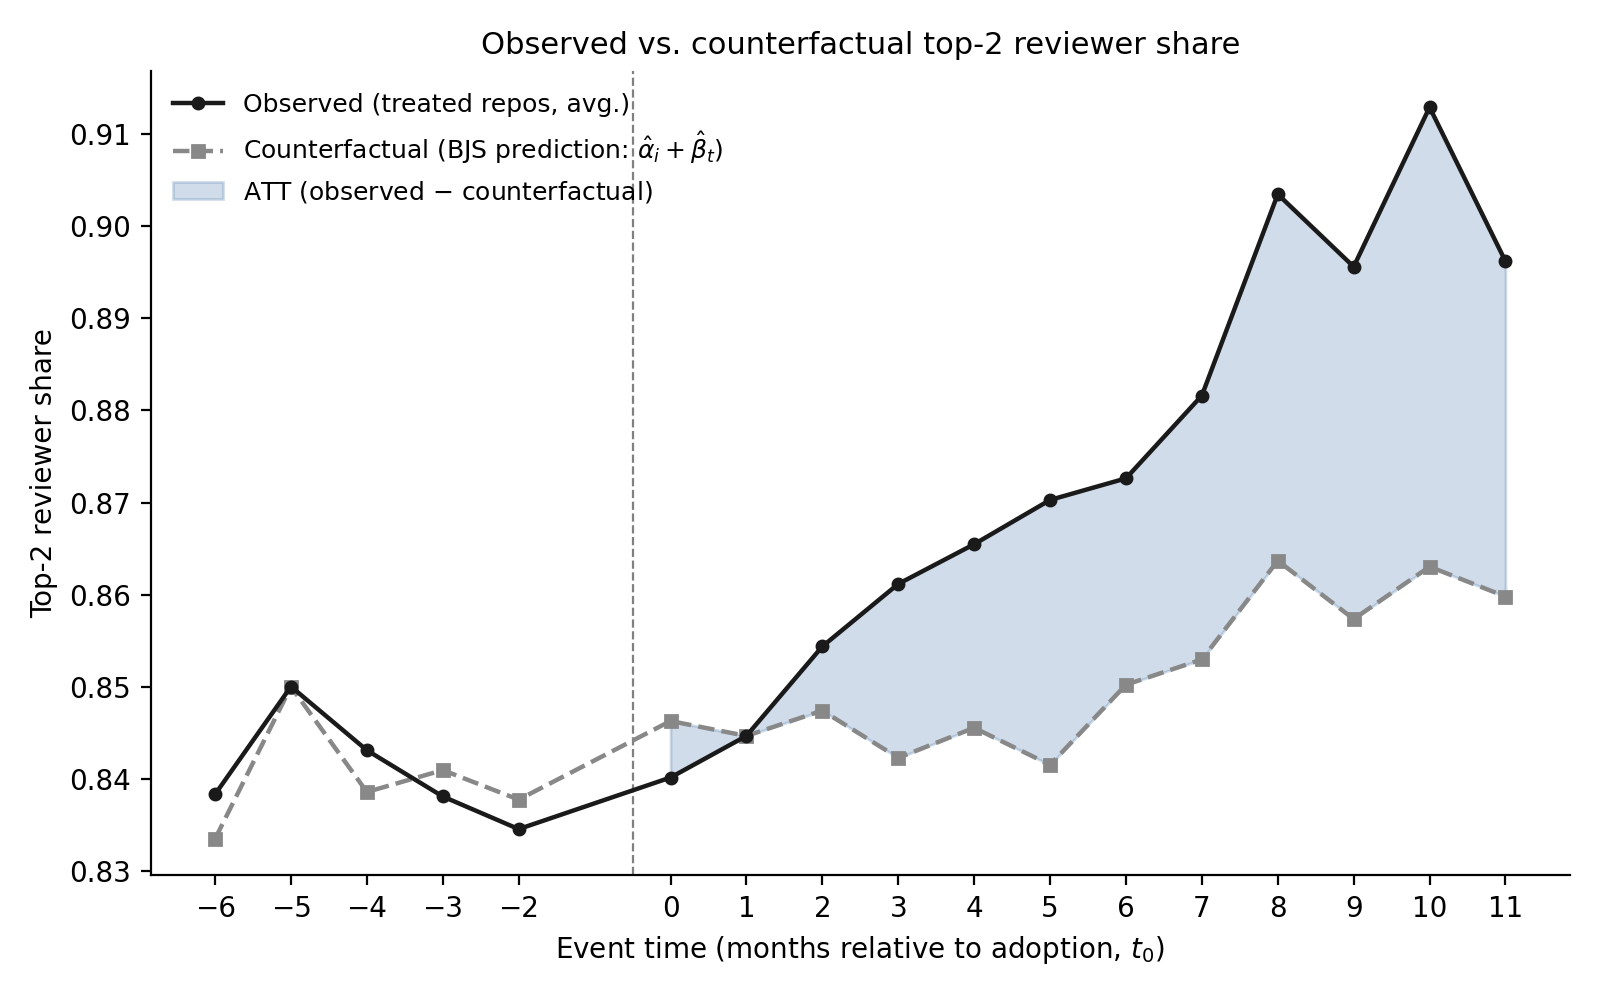
\includegraphics[width=0.85\textwidth]{figures/bjs_illustration_top2_share.png}
\end{center}
\end{frame}

\section{Results}

\begin{frame}{H1 --- Same People, Different Division of Labour}
\begin{table}
\centering
\small
\begin{tabular}{lrr}
\toprule
Outcome & ATT & $p$ \\
\midrule
Top-1 review share & $+0.017$ \ (0.0089) & 0.052 \\
Top-2 review share & $+0.015^{**}$ \ (0.0050) & 0.003 \\
Tail share (outside the top two) & $-0.015^{***}$ & $<0.001$ \\
Reviewer Gini coefficient & $+0.030^{***}$ & $<0.001$ \\
\addlinespace
\multicolumn{3}{l}{\textit{Repos with 3+ reviewers monthly}} \\
Top-1 review share & $+0.041^{***}$ \ (0.0072) & $<0.001$ \\
Top-2 review share & $+0.036^{***}$ \ (0.0052) & $<0.001$ \\
\addlinespace
Repo FE & Yes & \\
Time FE & Yes & \\
\bottomrule
\end{tabular}
\end{table}
\footnotesize All estimates above pass the pre-trend test; team size is unchanged. Gini computed on 1{,}406 of 1{,}771
pairs.
\end{frame}

\begin{frame}{H1 --- What the Numbers Show}
\begin{itemize}
  \item \textbf{Headcount:} team size is unchanged -- the group
        reassigns roles internally, it doesn't grow or shrink.
  \item \textbf{Concentration:} top-2 share rises while tail share
        falls by almost the same amount, and the Gini rises across the
        whole distribution -- work moves up within that fixed group,
        not just between the top two.
  \item Many repo-months start pinned near 100\% (only 1--2 reviewers),
        diluting the pooled estimate; restricting to 3+ reviewers
        roughly doubles it.
\end{itemize}
\vspace{0.3em}
\end{frame}

\begin{frame}{H1 --- Concentration Depends on Whether Leadership Was Already Settled}
Split treated repos by whether one person already held the top spot for
the entire 5-month pre-period (``settled'') or not (``unsettled''):
\begin{table}
\centering
\small
\begin{tabular}{lrr}
\toprule
Outcome & Unsettled leader ($n{=}191$) & Settled leader ($n{=}105$) \\
\midrule
Top-1 review share & $+0.047$ (4.62) & $-0.022$ ($-1.84$) \\
Top-2 review share & $+0.036$ (4.40) & $+0.001$ (0.14) \\
\bottomrule
\end{tabular}
\end{table}
\begin{itemize}
  \item Both strata pass pre-trend cleanly; the difference between them
        is strongly significant (top-1: $p<0.0001$, top-2: $p=0.003$).
  \item \textbf{Caveat:} tenure correlates with pre-adoption
        concentration level ($r=0.38$) -- the same confound flagged for
        the separate concentration-level split. Cannot yet separate a
        genuine threshold effect from mean reversion.
  \item \textbf{Scope:} this subsample (complete 5-month pre-period
        coverage) also skews busier than average ($\sim$2$\times$ the
        pre-period PR volume) -- a real subset, not the general
        population.
\end{itemize}
\end{frame}

\begin{frame}{H2 --- Reassigned, Not Destabilized}
\begin{table}
\centering
\small
\begin{tabular}{lrr}
\toprule
Outcome & ATT & $p$ \\
\midrule
Monthly leader is the pre-adoption top-1 & $-0.077^{***}$ \ (0.0151) & $<0.001$ \\
Monthly top-2 overlaps the pre-adoption top-2 & $-0.045^{***}$ \ (0.0101) & $<0.001$ \\
Month-to-month leader change & $-0.058^{**}$ \ (0.0197) & 0.004 \\
\addlinespace
Repo FE & Yes & \\
Time FE & Yes & \\
\bottomrule
\end{tabular}
\end{table}
\begin{itemize}
  \item The lead shifts to someone new relative to who led before
        adoption -- the shift builds gradually, not at once.
  \item Once that shift happens, it holds: month-to-month leader
        changes become \textbf{less} likely, not more -- one
        reassignment, then stability.
  \item \textbf{Caveat:} the first row is the robust driver of this
        result (survives and strengthens on the control-independence
        check, backup). The month-to-month row does not -- treat it as
        suggestive, not established.
\end{itemize}
\end{frame}

\begin{frame}{Is That Reassignment a Construction Artifact?}
The fixed identity is chosen by taking the maximum over
$h=-6,\dots,-2$, and those same months form the estimation baseline ---
which inflates pre-period persistence by construction.
\begin{center}
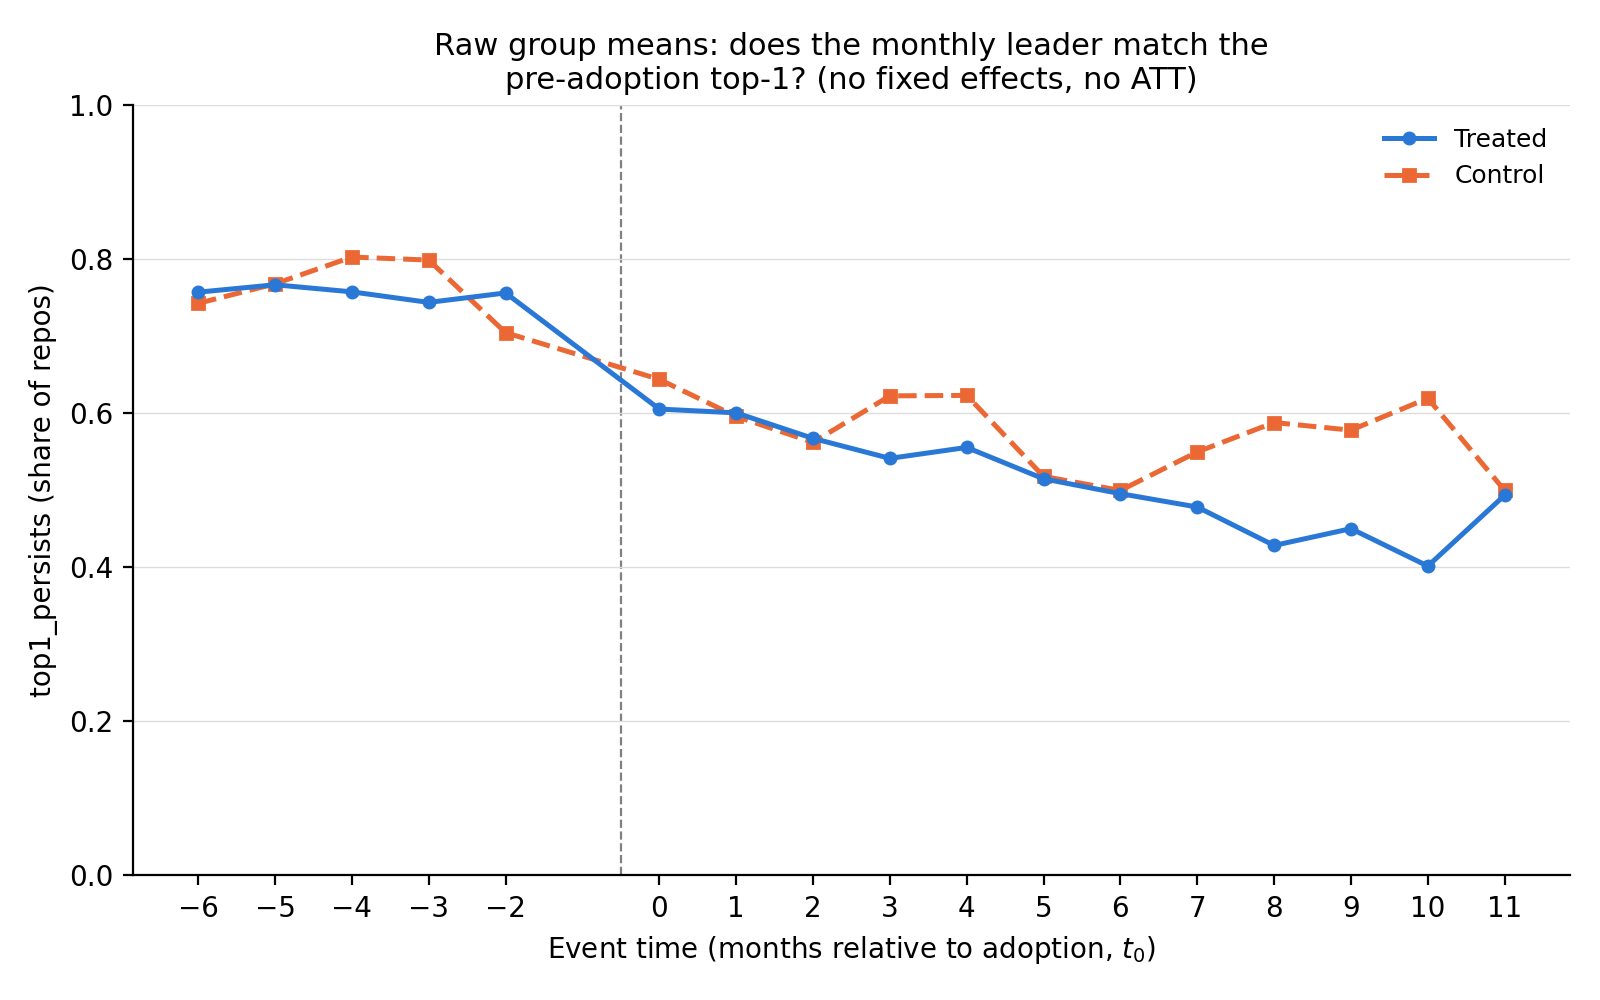
\includegraphics[width=0.72\textwidth]{figures/top1_persists_raw_event_time.png}
\end{center}
\vspace{-0.3em}
\footnotesize Both groups drop from $\sim$0.75 to $\sim$0.60 at
$h\!=\!0$: the artifact is real, and it is common to treated and
control, so the difference-in-differences nets it out. The treated
series separates only later.
\end{frame}

\begin{frame}{H3 --- The Process Signature}
\begin{table}
\centering
\small
\begin{tabular}{lrr}
\toprule
Outcome & ATT & $p$ \\
\midrule
Time to first review (h) & $-65.0^{*}$ \ (28.91) & 0.025 \\
Time to merge (h)        & $-62.8^{*}$ \ (27.10) & 0.021 \\
Review rounds/PR         & $+0.180^{*}$ \ (0.082) & 0.027 \\
\addlinespace
Repo FE & Yes & \\
Time FE & Yes & \\
\bottomrule
\end{tabular}
\end{table}
\begin{itemize}
  \item PRs reach review and merge sooner, but take more rounds to get
        there.
  \item Consistent with verification by someone carrying less
        project history: available sooner, needing more exchange to
        converge.
\end{itemize}
\end{frame}

\begin{frame}{H3 --- Do Pull Requests Just Get Smaller?}
\begin{table}
\centering
\small
\begin{tabular}{lrr}
\toprule
Spec & ATT (hours) & $t$ \\
\midrule
Unrestricted (uncapped PR-level data) & $-34.2$ & $-1.74$ \\
Residualized on PR size & $-35.8$ & $-1.82$ \\
Restricted to similarly-sized PRs (25th--75th pct.) & $-61.8$ & $-2.62$ \\
\bottomrule
\end{tabular}
\end{table}
\begin{itemize}
  \item With PR size held fixed, latency still falls --- merges get
        faster, not merely smaller.
\end{itemize}
\end{frame}

\begin{frame}{H3 --- Reverses in Busy Repos}
On the busier-than-average subsample ($\sim$2$\times$ pre-period PR
volume, $n{=}296$):
\begin{table}
\centering
\small
\begin{tabular}{lrr}
\toprule
Outcome & Full sample & Busy subsample \\
\midrule
Time to merge (h) & $-62.8$ (2.60) & $+40.7$ (2.83) \\
Review rounds/PR & $+0.180$ (4.04) & $-0.146$ (2.04) \\
\bottomrule
\end{tabular}
\end{table}
\begin{itemize}
  \item Both directions pass pre-trend, in both samples -- not a
        construction artifact. Checked and ruled out: $t_0$-timing
        bias, horizon-weighting (the full sample's own $\text{ATT}_h$
        never flips sign across any single horizon).
  \item In high-volume repos, merging gets \textbf{slower} and needs
        \textbf{fewer} rounds after adoption -- the opposite pattern
        from the general sample.
  \item Second independent signal (after H1's stronger-in-big-repos
        result) that large/busy projects respond qualitatively
        differently to AI adoption, not just more intensely.
\end{itemize}
\end{frame}

\section{Discussion}

\begin{frame}{What Changes When AI Arrives}
\begin{enumerate}
  \item \textbf{Same room, different seat}: headcount is unchanged;
        work moves from the periphery to the top.
  \item \textbf{The entry is reassigned, and it holds}: increasingly
        not the pre-adoption lead, widening gradually -- yet not more
        volatile, a rewritten directory.
  \item \textbf{Same signature in the process}: PRs reach review and
        merge sooner but take more rounds to converge.
\end{enumerate}
\vspace{0.4em}
A project's transactive memory can be reassigned by a tooling shock in
a matter of months, with membership constant --- and no throughput,
latency or participation metric registers it.
\end{frame}

\begin{frame}{The Traditional Model: Authority From Memory}
Code review has always run on one assumption: \textbf{the right
reviewer is whoever has accumulated the most memory of this specific
code.} This isn't folklore -- it's how the field has measured and
automated reviewer selection for over a decade.
\begin{itemize}
  \item Review's central function is building shared
        \emph{understanding} of the change, not just catching bugs
        \cite{bacchelli2013expectations}.
  \item State-of-the-art reviewer-recommendation tools formalize this
        directly: recommend whoever has reviewed similar file paths
        before \cite{thongtanunam2015revfinder}, or whoever has the
        deepest historical contribution to the changed files
        \cite{zanjani2016chrev}.
  \item Open-source peer review itself grew up as an informal,
        tenure-based norm -- whoever has been around long enough earns
        the authority to gate changes \cite{rigby2008apache}.
\end{itemize}
\vspace{0.3em}
The reviewer \emph{is} a gatekeeper \cite{allen1977gatekeepers} --
authority is durable, personal, and earned through years of
accumulated exposure to the codebase.
\end{frame}

\begin{frame}{Is That Model Breaking?}
Our own results, read together, say yes -- and we can be precise about
\emph{how}.
\begin{itemize}
  \item \textbf{Durable authority is dissolving into rotation.} A
        reviewer who led one half of the post-adoption window is no
        more likely to still lead the second half, treated vs.\
        control -- concentration is real, but it doesn't settle onto
        fixed individuals the way the traditional model predicts.
  \item \textbf{Suggestive, not yet established: a lower entry
        threshold.} Reassignment is strongest where tenure hadn't
        accumulated, weakest where a leader was already settled -- but
        this correlates (r=0.38) with those same repos' pre-adoption
        concentration level, a confound already flagged elsewhere.
        Can't yet separate a real threshold effect from mean reversion.
  \item \textbf{The apprenticeship pipeline that used to manufacture
        gatekeepers is thinning.} Peripheral, occasional reviewers --
        traditionally how someone earns the file-history that
        REVFINDER-style tools reward -- hold a shrinking share of
        activity.
\end{itemize}
\vspace{0.3em}
Put together: authority is shifting from \emph{accumulated, durable,
personal} to \emph{transient and capacity-based} -- whoever has
bandwidth this month, not whoever has the longest memory.
\end{frame}

\begin{frame}{Reconstructing the Process}
The standard pipeline (earlier slide) treats verification as a
discrete gate at the end: write, then check. That shape assumes
writing is the slow, scarce step.
\begin{itemize}
  \item AI inverts the economics: generating code is now nearly free.
        The bottleneck -- and the organizational weight -- moves
        almost entirely onto verification.
  \item A gate sized for the old economics cannot absorb that weight
        by staying a gate. Our data shows it isn't: the gate is
        already dissolving into a rotating, lower-threshold, less
        memory-dependent function.
  \item The traditional fix -- promote someone with years of context
        -- no longer matches how the role is actually being filled.
\end{itemize}
\vspace{0.3em}
\textbf{The reconstruction this implies:} verification has to become a
distributed, continuously-engineered property of the process, not a
checkpoint inherited from whoever has been there longest.
\end{frame}

\begin{frame}{What This Means in Practice}
\begin{itemize}
  \item \textbf{Stop indexing review capability by tenure.} If
        standing no longer takes years to earn, gatekeeping rules
        built around seniority (file ownership, CODEOWNERS-by-tenure)
        are already out of step with who is actually doing the work.
  \item \textbf{Track participation breadth, not just throughput.} A
        shrinking periphery is an early-warning signal -- like
        bus-factor -- invisible to every speed metric this paper also
        confirms is improving.
  \item \textbf{Engineer the apprenticeship pipeline deliberately.} It
        no longer forms for free; deliberate review-rotation for newer
        contributors has to replace what used to emerge organically.
  \item \textbf{Treat succession as a tracked risk, not an accident.}
        The handover already happens, usually without anyone planning
        it -- the open question is whether it happens \emph{to} a
        system designed for it.
\end{itemize}
\end{frame}

\begin{frame}{Are Our Controls Actually Independent?}
\textbf{Problem:} 37.7\% of repos share a human reviewer with some
treated repo elsewhere in the sample -- that reviewer can carry
AI-adoption habits into a repo we're counting as an untreated
``control,'' violating the no-interference assumption the design needs.
\vspace{0.3em}

\textbf{What we did:} identified the 176 fully independent (``clean'')
pairs and re-ran every headline outcome restricted to them.
\vspace{0.3em}

\textbf{Result if contamination is removed:}
\begin{itemize}
  \item \textbf{Survives and strengthens:} top-2 share, tail share,
        top1\_persists -- the paper's three most load-bearing results.
  \item \textbf{Weakens but same sign:} top-1 share, Gini, time-to-
        merge, review-rounds -- plausibly just power loss at $n{=}176$.
  \item \textbf{Does not survive:} month-to-month leader-change rate --
        collapses to $t{\approx}0$, dropped as a robust claim.
\end{itemize}
\end{frame}

\begin{frame}{Does It Matter Which AI Tool or Era?}
Tested two ways: \textbf{calendar-time adoption era} (proxy for tool
generation, since our signal can't identify model versions) and
\textbf{specific tool identity} (Codex, Copilot, Claude, Cursor).
\vspace{0.3em}
\begin{itemize}
  \item Neither split produces a significant difference in the
        concentration effect -- and that null survives the full
        battery: caliper sensitivity, bootstrap SE, and the clean-
        sample restriction above.
  \item One exception: Codex's own latency effect is individually
        robust (survives all three checks) -- but not provably larger
        than Copilot's or Claude's.
\end{itemize}
\vspace{0.3em}
\textbf{Reading:} the effect is general, not an artifact of any one
tool or AI generation -- a robustness result, not a new mechanism.
\end{frame}

\begin{frame}{Limitations}
\begin{itemize}
  \item \textbf{No downstream outcome}: We measure how verification is
        organized, not what it catches. Nothing here speaks to code
        quality, defects, or security.
  \item \textbf{Detection, not adoption}: $t_0$ is the first
        \emph{observed} signal; controls are never-detected rather than
        never-treated.
  \item \textbf{Merged PRs only}: What is never reviewed or never
        merged is outside the pipeline.
  \item \textbf{Entrant/incumbent share unusable}: The activity-level
        version fails the pre-trend test under the current 6-month
        pre-window definition, so we cannot yet say whether the
        reassigned lead is a long-standing member or a recent one.
  \item \textbf{Distinct-leaders-per-6-months not estimable}: the
        pre-period window (5 months) can never hold a full 6-month
        lookback, so no treated repo contributes pre-period data for
        this specific measure under the current design.
  \item \textbf{Gini not on the complete sample}: 1,406 of 1,771 pairs;
        the remaining 365 lack usable pre+post coverage in the
        repo-month cache, not a Gini-specific gap.
  \item \textbf{Controls are not fully independent}: a meaningful share
        of control repos share a reviewer with some treated repo, and
        this is worse precisely where the effect is strongest (backup).
\end{itemize}
\end{frame}

\begin{frame}{Future Work}
\begin{itemize}
  \item Redefine incumbency over full repository history (needs data
        before $h=-6$, a new extraction) and re-estimate the
        entrant/incumbent split -- the one measure that would close the
        ``who takes over'' question directly.
  \item Attach one downstream outcome (revert rate, post-merge defects,
        contributor retention) to connect structure to consequence --
        needs data types not currently collected.
\end{itemize}
\end{frame}

\begin{frame}[plain]
\begin{center}
\Large Thank you
\vspace{1em}

\normalsize Questions?
\end{center}
\end{frame}

\section{Backup}

\begin{frame}{Outcome Variables: Calculation Detail}
\textbf{top1\_share / top2\_share / tail\_share}: For each repo-month:
\begin{itemize}
  \item Count the distinct merged PRs reviewed by each human reviewer;
        each reviewer counted once per PR regardless of how many review
        events they submitted.
  \item Rank reviewers by this count. top1 is the highest individual
        count; top2 the combined count of the two highest; the tail is
        everyone else. Shares use the sum of all reviewers' counts as
        denominator.
\end{itemize}
\textbf{top1\_persists}: Freeze one identity per repository from the
pre-period only ($h=-6,\dots,-2$): the reviewer with the highest total
across those months. For every month, compare that fixed identity with
that month's busiest reviewer. Note this is a \emph{single person},
distinct from the monthly re-ranking used by top1\_share.
\vspace{0.3em}
\textbf{Reviewer Gini}: Per-PR reviewer identities reconstruct each
repo-month's complete reviewer-count distribution; the Gini of that
distribution (0 = equal split, 1 = one reviewer does everything)
replaces the earlier HHI approximation ($p=0.095$).
\end{frame}

\begin{frame}{Validating an Estimate Before Reporting It}
\begin{itemize}
  \item Parallel-trends check on the pre-period leads (next slide).
  \item Re-estimation at 5 matching calipers (0.10--0.50 SD). Tighter =
        fewer, closer-matched pairs; looser = more pairs, less precise
        matches. Caliper stability = does the result hold at every
        threshold, not just our main choice (0.25)?
  \item Balanced-panel restriction and a fixed 6-month common-horizon
        re-estimate (vs.\ the full 0--11 month window).
  \item Mean-reversion / selection-on-timing diagnostic.
  \item Repo-cluster bootstrap of the BJS standard errors.
  \item Adoption-signal precision re-check on newly collected data.
\end{itemize}
\vspace{0.5em}
An estimate that fails the pre-trend test is excluded from causal
interpretation, whatever its own significance. Two measures were
excluded this way: entrant share and total review count.
\end{frame}

\begin{frame}{Is the Reported Inference Trustworthy?}
Analytic cluster-robust SE vs.\ a 300-replicate repo-pair bootstrap:
\begin{table}
\centering
\scriptsize
\begin{tabular}{lrrrr}
\toprule
Outcome & Analytic SE & Bootstrap SE & Ratio & Corrected $p$ \\
\midrule
Top-1 review share     & 0.0064 & 0.0089 & 1.39$\times$ & 0.052 \\
Top-2 review share     & 0.0034 & 0.0050 & 1.45$\times$ & 0.003 \\
Time to first review   & 21.40  & 28.91  & 1.35$\times$ & 0.025 \\
Time to merge          & 24.18  & 27.10  & 1.12$\times$ & 0.021 \\
Review rounds          & 0.045  & 0.082  & 1.83$\times$ & 0.027 \\
\bottomrule
\end{tabular}
\end{table}
The analytic SE understates true uncertainty by 12--83\%. Top-1 share
drops to borderline ($p=0.052$); everything else survives. All tables
in this deck use the corrected $p$.
\end{frame}

\begin{frame}{The Parallel-Trends Assumption for BJS}
\begin{itemize}
  \item BJS builds each treated repo's counterfactual,
        $\hat\alpha_i+\hat\beta_t$, from a model fit only on
        pre-adoption and control data. That counterfactual is valid
        only if, absent treatment, the repo would have kept following
        that same repo-baseline-plus-calendar-trend path.
  \item Primary check (go/no-go): joint Wald test on the five
        pre-period lead coefficients ($h=-6,\dots,-2$), $\chi^2_5$.
  \item Secondary check (margin of safety): how large an undetected
        pre-trend would need to be, extrapolated forward, to explain
        away the post-period effect --- in units of the estimated
        pre-trend's own SE.
\end{itemize}
\begin{table}
\centering
\scriptsize
\begin{tabular}{lr}
\toprule
Outcome & Breakdown slope, in SE units \\
\midrule
Top-1 review share     & 2.6$\times$ (wrong-signed pre-trend --- helps us) \\
Top-2 review share     & 3.4$\times$ (wrong-signed pre-trend --- helps us) \\
Time to first review   & 3.7$\times$ (same-signed --- erodes $\sim$36\% of ATT) \\
Time to merge          & 3.8$\times$ \\
Review rounds          & 3.0$\times$ (same-signed --- erodes $\sim$55\% of ATT) \\
\bottomrule
\end{tabular}
\end{table}
\end{frame}

\begin{frame}{Robustness Check}
\begin{table}
\centering
\scriptsize
\begin{tabular}{lll}
\toprule
Outcome & Caliper stability (5 tested) & Mean-reversion \\
\midrule
Top-1 review share     & Stable, all 5 calipers & No concern \\
Top-2 review share     & Stable, all 5 (fails pre-trend at 1) & No concern \\
Time to first review   & Stable, all 5 calipers & Mild caveat \\
Time to merge          & Stable, all 5 calipers & Caveat (asymmetry) \\
Review rounds          & Stable 5/5, sig.\ 4/5 (fails pre-trend at 1) & No concern \\
\bottomrule
\end{tabular}
\end{table}
\vspace{0.5em}
\scriptsize No outcome above changes sign at any caliper. Outcomes that
failed validation (raw top-1 review count, entrant share, total review
count) are excluded from causal interpretation.
\end{frame}

\begin{frame}{Is the Full-Window Effect a Cohort Artifact?}
Treated observations shrink from 1,405 at $h{=}0$ to 205 at $h{=}11$ ---
later horizons rest on a smaller, longer-surviving subset of repos.
\begin{table}
\centering
\scriptsize
\begin{tabular}{lrr}
\toprule
Outcome & Full ATT & Common-horizon ATT ($h=0..5$) \\
\midrule
Top-1 review share     & $+0.0173$ & $+0.0075$ \\
Top-2 review share     & $+0.0151$ & $+0.0081$ \\
Time to first review   & $-65.0$   & $-53.1$ \\
Time to merge          & $-62.8$   & $-56.9$ \\
Review rounds          & $+0.180$  & $+0.177$ \\
\bottomrule
\end{tabular}
\end{table}
Concentration's full-window ATT is roughly double the common-horizon
estimate --- part of the apparent late-horizon growth is cohort
composition, not pure treatment dynamics. Since the reassignment effect
in H2 also grows with horizon, the same check is owed for
top1\_persists.
\end{frame}

\begin{frame}{Caveat: A Sampling Cap in the Repo-Month Extraction}
\begin{itemize}
  \item The original repo-month pipeline capped each repo-month at 40
        sampled merged PRs (binds for $\sim$11\% of repo-months). The
        new PR-level extraction has no such cap.
  \item Re-estimating H1 on the identical 802-repo subsample:
\end{itemize}
\begin{table}
\centering
\small
\begin{tabular}{lrr}
\toprule
Outcome & Capped ATT ($t$) & Uncapped ATT ($t$) \\
\midrule
Top-1 review share & $+0.0141$ (2.07) & $+0.0070$ (1.12) \\
Top-2 review share & $+0.0153$ (4.08) & $+0.0082$ (2.47) \\
\bottomrule
\end{tabular}
\end{table}
\begin{itemize}
  \item The cap roughly \textbf{doubles} the concentration point
        estimates where it binds --- top-1 share loses significance
        uncapped, top-2 share survives ($t=2.47$).
  \item Direction is not overturned; the full-sample effect size is
        probably somewhat inflated.
\end{itemize}
\end{frame}

\begin{frame}{Caveat: Controls Are Not Fully Independent}
\begin{itemize}
  \item 37.7\% of repos share a reviewer with some treated repo
        elsewhere in the sample (identity-covered subsample, 309 pairs)
        -- a SUTVA violation. Over half of contaminated repos are
        contaminated via their own \emph{lead} reviewer, not a
        peripheral one.
  \item This is a popular-project effect, not a small-project one:
        contaminated repos have 2$\times$ the reviewer pool of clean
        repos (median 10 vs.\ 5) and more stars/contributors.
\end{itemize}
\begin{table}
\centering
\small
\begin{tabular}{lrr}
\toprule
Outcome & Contaminated-only ($t$) & Clean-only ($t$) \\
\midrule
Top-1 review share & $+0.0376$ (2.46) & $+0.0118$ (0.86) \\
Top-2 review share & $+0.0462$ (4.77) & $+0.0208$ (2.79) \\
\bottomrule
\end{tabular}
\end{table}
\begin{itemize}
  \item The effect is \textbf{stronger}, not weaker, in the
        contaminated segment -- consistent with the 3+-reviewer
        subgroup result, but it means the strongest part of the signal
        sits exactly where control independence is most in question.
  \item Cannot yet separate a genuinely larger effect in bigger/more-
        interconnected projects from inflation due to non-independent
        controls there.
\end{itemize}
\end{frame}

\begin{frame}{Does the Effect Differ by Adoption Era?}
Repos adopted 2025-05 to 2025-11 (``Era 2'', $n{=}413$) vs.\
2025-11 to 2026-05 (``Era 3'', $n{=}666$) -- the two best-powered
calendar-time cohorts, roughly bracketing successive generations of
agentic coding tools:
\begin{table}
\centering
\small
\begin{tabular}{lrrl}
\toprule
Outcome & Era 2 ATT & Era 3 ATT & Diff.\ test \\
\midrule
Top-1 review share & $+0.028$ & $+0.020$ & $p=0.60$ \\
Top-2 review share & $+0.021$ & $+0.014$ & $p=0.42$ \\
\bottomrule
\end{tabular}
\end{table}
\begin{itemize}
  \item No test in a full battery -- caliper sensitivity, bootstrap
        SE, clean-sample restriction -- ever produces a significant
        Era-2-vs-Era-3 difference on this comparison.
  \item \textbf{The effect is not detectably different across adoption
        eras.} Not driven by a specific generation of AI coding tools.
\end{itemize}
\end{frame}

\begin{frame}{Caveat: Era-Specific Estimates Are Individually Fragile}
Same robustness battery applied to each era's own ATT, not just the
Era-2-vs-Era-3 comparison:
\begin{itemize}
  \item \textbf{Caliper:} only 2 of 4 era$\times$outcome cells are
        sign-stable across all 5 calipers -- and Era 2's stable
        outcome isn't the same as Era 3's.
  \item \textbf{Bootstrap (300 reps, within era):} knocks out 3 of 4
        originally-significant cells; only Era 2's top-2 share
        survives ($t=2.12$, $p=0.034$).
  \item \textbf{Clean sample:} none of the 4 cells survive (small
        cells, $n{=}49$/$78$).
\end{itemize}
\vspace{0.3em}
Read carefully: this does \textbf{not} contradict the no-era-difference
finding above -- both eras lose significance under the same pressures,
roughly equally, which is itself consistent with ``no era-specific
effect.'' But splitting into era cohorts should not be cited as two
independently robust confirmations of the headline result; it mostly
reduces $n$ and reproduces known fragility (contamination sensitivity,
caliper sensitivity) already documented elsewhere in this deck.
\end{frame}

\begin{frame}{Does the Effect Differ by Specific Tool?}
Beyond agent-vs-assisted MODE (earlier slide): does it matter whether a
repo adopted Codex, Copilot, Claude, or Cursor specifically? Buckets are
non-exclusive (a repo can carry signals for more than one tool).
\begin{table}
\centering
\small
\begin{tabular}{lrrr}
\toprule
Tool ($n$) & Top-2 share $t$ & Time-to-merge $t$ \\
\midrule
Codex (961)    & $+1.57$ & $-2.97$ \\
Copilot (800)  & $+3.18$ & $-2.60$ \\
Claude (478)   & $+2.55$ & $-1.26$ \\
Cursor (151)   & $+0.66$ & $+1.10$ \\
\bottomrule
\end{tabular}
\end{table}
\begin{itemize}
  \item No pairwise diff-in-ATT among Codex, Copilot, and Claude --
        the three well-powered buckets -- ever reaches significance,
        on either outcome, even after bootstrap correction.
  \item \textbf{No detectable difference by specific tool among the
        buckets with enough power to test.} Consistent with the
        adoption-era finding: the effect is general, not tool-specific.
\end{itemize}
\end{frame}

\begin{frame}{Caveat: Per-Tool Estimates Are Individually Fragile Too}
Same robustness battery applied to each tool's own ATT:
\begin{itemize}
  \item \textbf{Top-2 share: fragile for ALL FOUR tools.} Sign flips
        across the 5 calipers for every single bucket, including
        Copilot and Claude, which looked individually significant at
        the main caliper -- the same matching-artifact signature used
        elsewhere in this deck to reject a result.
  \item \textbf{Time-to-merge is more stable}, and \textbf{Codex's own
        estimate is the one genuinely robust per-tool result here}:
        sign-stable across all 5 calipers, survives bootstrap
        ($t=-2.06$), survives the clean-sample restriction
        ($t=-2.65$, $n{=}85$). Not provably \emph{larger} than
        Copilot's or Claude's effect, though -- just the cleanest on
        its own terms.
  \item Cursor's apparent differences (wrong-signed point estimates,
        the only significant pairwise comparisons) trace to a small,
        caliper-unstable, not-individually-significant bucket -- the
        same ``apparent difference is really just one noisy slice''
        pattern as Era 4's truncated panel, not a real tool effect.
\end{itemize}
\vspace{0.3em}
Read together with the adoption-era result: splitting the pooled
headline findings by any single covariate -- era or tool -- mostly
costs power and reproduces known fragility, rather than revealing a
real source of heterogeneity.
\end{frame}

\begin{frame}{Where Exactly Does the Share Go?}
Full rank-by-rank breakdown (uncapped, full sample) -- not just
top1/top2/tail:
\begin{table}
\centering
\small
\begin{tabular}{lrrr}
\toprule
Rank & ATT & $t$ & Pre-trend \\
\midrule
1 (busiest) & $+0.0066$ & 1.06  & Pass \\
2            & $-0.0078$ & $-1.73$ & Pass \\
3            & $-0.0127^{***}$ & $-4.19$ & Pass \\
4            & $-0.0083^{***}$ & $-3.68$ & Pass \\
5            & $-0.0041^{*}$  & $-2.24$ & Pass \\
\bottomrule
\end{tabular}
\end{table}
\begin{itemize}
  \item Not a clean ``top gains'' story: the single busiest reviewer
        barely moves on this cut. The real, significant losses sit at
        ranks 3--4 -- the moderately-active middle, not the top and
        not just the deep periphery.
  \item Rank 1+2 combined is roughly flat here ($\approx -0.001$) --
        in tension with the capped-pipeline top2\_share headline
        ($+0.015$). A third, independent confirmation of the sampling-
        cap caveat (next slide), not a new separate issue.
  \item Best current read: the moderately-active middle hollows out,
        while the very top holds roughly steady -- a more precise, and
        different, story than ``work piles onto the top two.''
\end{itemize}
\end{frame}

\begin{frame}{Robustness to Control Independence: Full Table}
All 10 headline outcomes, re-estimated on the 176 reviewer-independent
("clean") pairs vs.\ the full sample. All 10 pass pre-trend on the
clean sample -- not a construction artifact.
\begin{table}
\centering
\scriptsize
\begin{tabular}{lrrl}
\toprule
Outcome & Full $t$ & Clean (176) $t$ & Verdict \\
\midrule
Top-1 share            & 1.91  & 0.86  & Weakens \\
Top-2 share             & 3.00  & 2.79  & \textbf{Survives, strengthens} \\
Tail share               & $-3.00$ & $-2.79$ & \textbf{Survives, strengthens} \\
Reviewer Gini            & ---   & 1.49  & Weakens \\
top1\_persists            & $-5.10$ & $-3.70$ & \textbf{Survives, strengthens} \\
top2\_overlap             & $-4.46$ & 0.45  & Null (not a confident reversal) \\
Month-to-month leader change & $-2.95$ & $-0.02$ & \textbf{Collapses} \\
Time to first review     & $-2.25$ & $-2.92$ & Survives, strengthens \\
Time to merge             & $-2.32$ & $-1.88$ & Weakens \\
Review rounds              & 2.20  & 1.82  & Weakens (sign holds) \\
\bottomrule
\end{tabular}
\end{table}
\begin{itemize}
  \item The paper's two most load-bearing rows -- top-2 share and
        top1\_persists -- are also the most robust.
  \item Month-to-month leader change does not survive; drop it from any
        claim of robustness, report top1\_persists as H2's driver.
\end{itemize}
\end{frame}

\begin{frame}{Does the Adoption Mode Matter?}
Agent-authored PRs vs.\ human-committed AI-assisted trailers only,
bootstrap-corrected difference test:
\begin{table}
\centering
\scriptsize
\begin{tabular}{lrrl}
\toprule
Outcome & Agent ATT & Assisted ATT & Difference \\
\midrule
Top-1 share    & $+0.010$ (n.s.) & $+0.039^{*}$    & $p=0.114$ (n.s.) \\
Top-2 share    & $+0.009$ (n.s.) & $+0.033^{***}$  & $p=0.037$ \\
Time to 1st review & $-57.3$ (n.s.) & $-73.6^{*}$  & $p=0.75$ (n.s.) \\
Time to merge  & $-67.2^{*}$     & $-43.4$ (n.s.)  & $p=0.60$ (n.s.) \\
Review rounds  & $+0.24^{*}$     & $-0.01$ (n.s.)  & $p=0.096$ (n.s.) \\
\bottomrule
\end{tabular}
\end{table}
Only the top-2-share difference survives correction ($p=0.037$). We
treat ``adoption mode matters'' as suggestive, not established.
\end{frame}

\begin{frame}{Robustness Check: Does the Result Vary by Team Size?}
Repos split into small-pool and large-pool halves by pre-adoption
reviewer count:
\begin{table}
\centering
\scriptsize
\begin{tabular}{lrrl}
\toprule
Outcome & Small-pool ATT & Large-pool ATT & Diff.\ test \\
\midrule
Time to 1st review & $-53.2$ (n.s., fails pre-trend) & $-80.0$ (n.s.) & $p=0.65$ \\
Time to merge      & $-64.8^{*}$                     & $-56.7$ (n.s.) & $p=0.89$ \\
Review rounds      & $+0.28^{**}$ (fails pre-trend)  & $+0.08$ (n.s.) & $p=0.28$ \\
\bottomrule
\end{tabular}
\end{table}
H3's process results hold whether the starting team was small or large.
One split that looked significant before correction (small pools,
review rounds) disappeared once properly tested.
\end{frame}
% \include{part2}

\begin{frame}[allowframebreaks,noframenumbering]{References}
    \printbibliography[heading=none]
\end{frame}

\end{document}